\section{Introduction}

The GitHub issue resolution task aims to automatically resolve a wide variety of issues proposed by developers in code repositories. These issues include diverse tasks such as fixing bugs, adding new features, refactoring code, writing documentation, etc~\cite{BissyandeLJRKT13,TaoZWZWZ24}. Effectively addressing these issues is crucial for maintaining and evolving real-world software systems. With the development of large language models (LLMs), 
this task has gained increasing attention~\cite{xia2024agentless,liu2024marscode,tao2024magis,yang2024swe,chen2024coder,zhang2024autocoderover,arora2024masai,wang2024opendevin,ma2024understand}.
%researchers have made some progress in using these models to automatically resolve real issues in code repositories~\cite{tao2024magis,xia2024agentless,liu2024marscode,yang2024swe,chen2024coder,zhang2024autocoderover}

Several benchmarks~\cite{zan2024swe,jimenez2023swe,openai2024swe,aleithan2024sweplus} currently exist for the GitHub issue resolution task. SWE-bench~\cite{jimenez2023swe} is the first benchmark in this area, consisting of 2,294 real-world issues from 12 Python repositories. Subsequently, OpenAI proposes SWE-bench Verified~\cite{openai2024swe}, a subset of SWE-bench with 500 instances verified by experienced developers to provide a more robust evaluation. Additionally, SWE-bench-java~\cite{zan2024swe} is introduced to extend the task to the Java programming language, including 93 task instances from 6 Java repositories.  Although various benchmarks have been proposed, there are still some limitations that prevent them from fully capturing the diversity of real-world issue resolution tasks. The primary limitations are as follows:

%Moreover, SWE-bench Multimodal collects 617 issues from 17 JavaScript repositories to evaluate issue resolution ability of LLMs with images as visual inputs.

\begin{itemize}[left=10pt]
    \item \textbf{L1: Focusing on a Single Programming Language.} Existing benchmarks typically focus on issues from repositories in a single programming language, such as Python or Java, which limits their capacity to assess the LLMs' ability to resolve issues across multiple programming languages.

    % evaluating the ability of LLMs to resolve issues across repositories in different languages.
    % Previous benchmarks typically focus on issues from repositories in a single programming language, such as Python or Java. This limits the usage of these benchmarks to evaluate the multilingual issue resolution ability of LLMs.


    \item \textbf{L2: Limited Repository Diversity.} Current benchmarks, such as SWE-bench~\cite{jimenez2023swe}, largely rely on issues from a limited range of domains, e.g., scientific computing, machine learning, and visualization. To better represent real-world issue resolution tasks, more repositories from a wider variety of domains are needed.

   \item \textbf{L3: Ignoring Multimodal Information.} Previous benchmarks focus solely on textual information in issue descriptions, overlooking multimodal information. Users often use images, such as screenshots of error messages or debugging outputs, to help illustrate issues more clearly. %\hy{can say it better} \glh{revised}.  
   Without incorporating this information, LLMs may have difficulty fully understanding the issue, leading to inaccurate evaluations. %\hy{can say why mutlimodal data such as images are needed for solving github issues} \hy{can describe what images they are about.} \glh{revised again}


\end{itemize}


% The GitHub issue resolution task aims to automatically resolve issues proposed by developers in code repositories, which is of great significance for real-world software maintenance and evolution. With the development of large language models (LLMs), researchers attempt to use these models to automatically resolve real issues in code repositories. 
% However, solely relying on LLMs has shown suboptimal performance on this task. Consequently, several retrieval-augmentation and multi-agent-based methods are proposed to enhance the performance of LLMs in this chanllenging task.



% Researchers have introduced various benchmarks for this task. For instance, Jimenez et al. proposed SWE-Bench, which includes 2,294 resolved GitHub issues collected from 12 Python repositories, along with execution environments to evaluate the correctness of submitted fixing patches. Later, OpenAI released SWE-Bench-Verified, a subset of SWE-Bench containing 394 task instances that are manually verified by experienced developers. In addition, Zan et al. introduce SWE-Bench-Java, collecting 94 resolved GitHub issues from 6 Java repositories as task instances.


% However, existing benchmarks face several limitations:  \textbf{(1) focusing on a single programming language}, \textbf{(2) overlooking diverse information of different modalitys in issues}, \textbf{(3) lacking diversity in repository domains}. 

% However, current datasets typically evaluate model performance on repositories of a single programming language, limiting the ability to evaluate multilingual issue-resolving capabilities of LLMs. 

%To fill this gap, 
In this paper, we present \textbf{\Swebenchx}, a benchmark for \textbf{G}itHub \textbf{I}ssue \textbf{R}eso\textbf{L}ution that incorporates multiple aspects of diversity in programming languages, repository domains and modality of input information. %the first multilingual issue resolution %\hy{what is "multilingual issue resolution"? an issue associated with many PLs? or issues of software written in multiple PLs? or just issues of software of different PLs?}\glh{the third one, i try to make it clear.} 
%benchmark  with multimodal inputs, covering 7 different domains.
We first select four most popular programming languages (i.e., Python, TypeScript, JavaScript, and Java) as target languages,\footnote{\url{https://github.blog/news-insights/research/the-state-of-open-source-and-ai/}} and collect a candidate list of the most widely used repositories based on download counts from package management tools (i.e., pip~\cite{pip}, npm~\cite{npm}, maven~\cite{maven}). From this candidate list, we select 15 repositories %\hy{SWE-bench contains 12 repos, 15 does not look many. also, do these 15 repos overlap with the previous 12 repos? also, 15 for 4PLs does not sound many (small-scale?)}\glh{The 15 repos in our benchmark do not have overlap with repos in SWE-bench. As to the number of repos, maybe i should mention this in Threats to Validity.}
from various domains and collect real-world issues from these repositories to construct task instances. After validating the collected task instances, we obtain a total of 959 task instances covering a variety of domains %\hy{how many domain do existing benchmarks cover? is 7 a lot?}
in four programming languages (addressing \textbf{L1} and \textbf{L2}). In addition to textual information in issue descriptions, we find some issues include other modalities. For instance, users use images, such as screenshots of error messages, to describe issues more clearly.  We manually examine issue descriptions on \Swebenchx and identify 19 instances containing images providing crucial information for resolving the issues. %\hy{why these images are crucial?}. \glh{I use 'necessary' and add explanation in the former sentence.}\hy{what images, and why "crucial/necessary"?}
% This subset is referred to as \textbf{SWE-Bench-Visual}
%\hy{not sure if a different benchmark name is needed}\glh{revised, delete this name}, 
%designed to evaluate the multimodal issue resolution capabilities of LLMs. 
Moreover, we find that users sometimes share website links to online code platforms, which typically contain code reproducing the issue.  We annotate these links in the dataset, offering future researchers the opportunity to explore how to leverage such resources to enhance issue resolution performance (addressing \textbf{L3}).




% We collect a total of xxx resolved issues from 15 GitHub repositories in four programming languages (i.e., Python, TypeScript, JavaScript, and Java). Additionally, we construct execution environments manually for each task instance to enable accurate evaluation. Moreover, we identify some GitHub issues in the dataset where the description includes visual information, such as images. We filter these task instances and created \textbf{SWE-Bench-Visual} to provide a more comprehensive evaluation of models' issue-resolving abilities.

% 补充一些数据集的特性

% Moreover, we evaluate multi-lingual issue resolution capabilities of current advanced LLMs on our dataset using the Agentless~\cite{xia2024agentless} framework. The experimental results show that xxx achieved a score of xx, setting a new state-of-the-art (SOTA) performance. However, we observed that LLMs perform worse on JavaScript and Java compared to Python, indicating the need for improvement in their issue-resolving capabilities across different programming languages.

We evaluate state-of-the-art LLMs on \Swebenchx, and the results show that the best-performing method, \GPT with the Agentless-X approach,\footnote{Because the Agentless~\cite{xia2024agentless} method is designed for Python language, we extend this method to other programming languages without changing the key design of this method. The multilingual version of this method is called Agentless-X.} resolves only 8.6\% of issues, highlighting the challenges of resolving issues from repositories in multiple languages. Additionally, we observe that the Agentless-X method performs worse on TypeScript and JavaScript tasks than Java and Python. Besides, we evaluate two advanced LLMs with visual abilities in the task instances with images as visual inputs, with \Claude achieving a best resolve rate of only 10.5\% and \GPT achieving just 1.6\%. The results show that both LLMs show limited performance on issues requiring understanding images.
% Besides, we evaluate LLMs in issues with visual inputs, the results show that

%We evaluate state-of-the-art LLMs on \SwebenchX, and the results show that the best pef

%补充实验结果的分析，模型哪里做的不好？

% Finally, to explore which characteristics of issues make them difficult for LLMs to resolve, we collect various information about the issues, such as resolution time, and calculated their correlation with the success rate of the models. The analysis revealed that: (1) xx can effectively indicate issue difficulty; (2) ...

Finally, we analyze the reasons why LLMs fail to resolve issues on \Swebenchx. First, we observe that when using the Agentless method, \Claude often struggles to generate outputs that follow the specified format outlined in the prompt. This formatting issue leads to intermediate results that cannot be parsed correctly, preventing the generation of patches in the next stage. As a result, \Claude achieves a low issue resolve rate of only 1.9\% on \Swebenchx. However, we find that the resolve rate increases to 7.4\% by modifying the prompt simply. Second, we find that the current LLMs have a significantly lower resolve rate on issues that require modifications across multiple files compared to those requiring single-file changes. Besides, for issues needing multi-file modifications, we find models tend to modify a single file, highlighting a limitation in the cross-file issue resolution capabilities of LLMs.

In summary, our contributions are as follows:


\begin{itemize}[left=10pt]
    % \item We introduce the first multilingual issue-resolving dataset called \Swebenchx and create SWE-Bench-Visual, a subset with visual inputs.
    \item We introduce \Swebenchx, a GitHub issue resolution benchmark with multi-aspect diversity in programming languages, repository domains and modality of input information. 
    % \item We evaluate LLMs' issue resolving abilities on \Swebenchx, revealing that current models lack sufficient issue resolving capabilities across different languages.

    \item We evaluate LLMs' issue resolving abilities on \Swebenchx, revealing that current models demonstrate limited overall performance across multiple programming languages.
    
    \item We evaluate LLMs' performance on issues that require visual information, revealing their limited capability in resolving issues with multimodal inputs.

    \item We conduct an analysis to investigate the reasons why LLMs fail to resolve issues, providing insights for improving issue resolving performance of LLMs in the future.
    % \item We investigate which characteristics of issues influence the difficulty of resolving them with LLMs.
\end{itemize}

% \hy{a related work: Qinkai Zheng, et al., Codegeex: A pre-trained model for
% code generation with multilingual benchmarking on humaneval-x. In Proceedings of the 29th
% ACM SIGKDD Conference on Knowledge Discovery and Data Mining, pp. 5673–5684, 2023b.} \glh{added in related work}



\begin{table}[t]
\centering
\footnotesize
\setlength\tabcolsep{3pt}
\caption{Overview of existing GitHub issue resolution datasets. }
\tabmargin
% \vspace*{-10pt}
% \multicolumn{4}{c}{\textbf{\revise{Metric}}
% \resizebox{\columnwidth}{!}{
% |c|c|c|c|c|c
    \begin{tabular}{lccccccc}
    \toprule
    \multirow{2}{*}{\textbf{Dataset}} & \multirow{2}{*}{\textbf{Year}} & \multicolumn{4}{c}{\textbf{Programming Languages}} & \multirow{2}{*}{\textbf{\# Repositories}} & \multirow{2}{*}{\textbf{\# Instances }} & \textbf{w/ Visual} \\
    \cmidrule(r){3-6}
    && \bf Python & \bf Java & \bf TypeScript & \bf JavaScript & & & \bf Input\\
    \midrule
    % \hline
    SWE-bench~\cite{puri2021codenet} & 2023 & $\checkmark$ & $\times$ & $\times$& $\times$& 12 & 2,294 & $\times$ \\
    % \hline
    SWE-bench-Java~\cite{ahmad2021avatar} & 2024 & $\times$& $\checkmark$ & $\times$& $\times$&6 & 91 & $\times$  \\
    % \hline
    SWE-bench-Verified~\cite{liu2024your} & 2024 & $\checkmark$ &$\times$ &$\times$ &$\times$ &12& 500 & $\times$  \\
    \midrule

    \Swebenchx &2024& $\checkmark$ & $\checkmark$ & $\checkmark$ &$\checkmark$ & 15 & 959 & $\checkmark$  \\
    \toprule
\end{tabular}
% }%
\label{table:datasets}
    % SWE-Bench-Multimodal~\cite{yan2023codescope} &2024& Javascript & 17 & 617 & Yes  \\
    % \hline
% \vspace*{-2em}
\end{table}%

\secmargin
\section{Background and Related Work}

% \begin{wrapfigure}{r}{0.7\textwidth}
\begin{figure}[t]
    \centering
    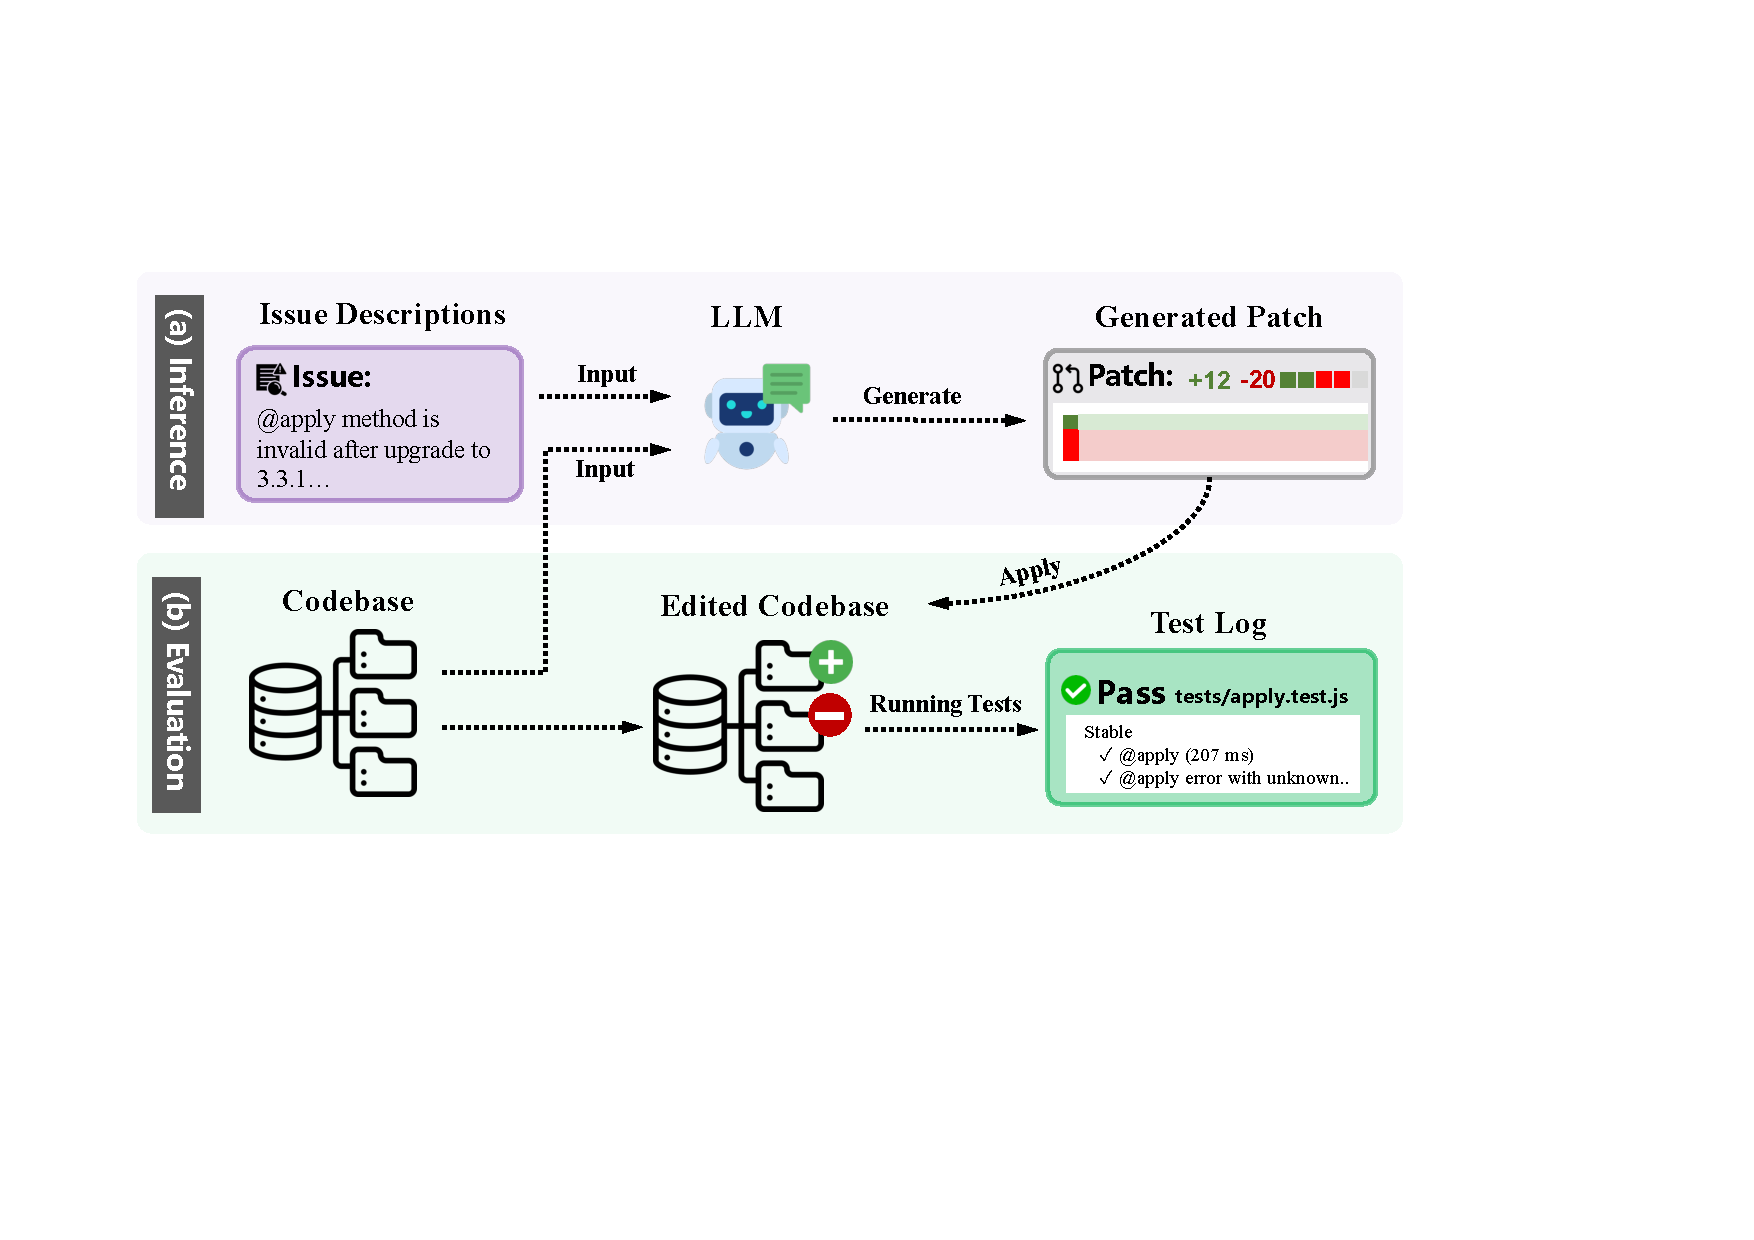
\includegraphics[width=0.8\linewidth]{figures/EvaluationPipelineV3.pdf}
    \figmargin
   \caption{Overview of the evaluation pipeline of GitHub issue resolution.}%\hy{not clear if this figure is needed}}
    \label{fig:TaskDefinition}
\end{figure}
% \end{wrapfigure}

\subsection{GitHub Issue Resolution}
% \hy{where is the definition? what task? Also perhps no need to use subsections here.} \glh{revised, do not use subsections here}\hy{can merge it with Section 3, Section 2: Background and Related Work
% Section 2.1 GitHub Issue Resolution}\glh{revised}
The GitHub issue resolution task aims to resolve issues reported in the GitHub repository automatically~\cite{jimenez2023swe,zan2024swe}. % \subsection{Pipeline of Evaluation}
When evaluating the issue resolution ability of LLMs, %\hy{what does it want to say?}\glh{here i wanna introduce the process of evaluating LLMs in issue resolution task.} 
we follow the pipeline as shown in Figure~\ref{fig:TaskDefinition}. In the inference stage, the LLMs receive the issue descriptions and the corresponding codebase, and generate a patch containing all code changes to the original codebase. In the evaluation stage, the generated patch is applied to the codebase, and all test cases related to this issue are run. After obtaining the test log, we check the statuses of the test cases. The issue is considered resolved if all related test cases pass successfully. Some key concepts are listed below:
%we input the issue descriptions and codebase to the LLMs, and generate a patch containing all code changes to the original codebase. In the evaluation stage, we apply the generated patch to the codebase and then run tests related to this issue. After obtaining the test log, we check the statuses of the test cases. We consider the issue resolved only if all related test cases pass successfully. 
% As shown in Figure~\ref{fig:TaskDefinition}, this task typically contains descriptions of an issue as input and expects to output code changes to fix this issue. To evaluate generated results automatically, this task verifies the correctness of results by running specialized tests. 

\begin{itemize}%[left=10pt]
    \item \textbf{Issue Descriptions:} descriptions about reported issues in the format of texts or images. 
    \item \textbf{Generated Patch:} a generated file including all code changes in the code repository to resolve reported issues. All code changes are formatted in the GitHub diff format.
    \item \textbf{Codebase:} the code repository contning the reported issue and all relevant code files necessary for resolving the issue.
    \item \textbf{Test Log:} a log file containing all test results, which is used to verify the correctness of results.
\end{itemize}





%\subsubsection{The inference stage.} \subsubsection{The evaluation stage.}   In this process, the issue descriptions provide the requirements for resolving issues, and the codebase provides relevant code context for making code changes. 



% \section{Related Work}
\subsection{LLM-based Methods for GitHub Issue Resolution}


% Github issue resolution是一个重要的软件维护活动。In popular GitHub repositories,  tens or hundreds of issues are reported daily\cite{}. Isuee submmiter report new issue 去汇报仓库潜在的bugs，询问仓库相关问题，提出新的特性等。随后开发者会尝试修复reported issue，并将修改的内容通过pull request上传到repo。仓库的管理者随后会对这些pull request进行验证，并决定是否合并。通过这个过程，仓库可以保持持进化。然而这也是一个对开发者十分有挑战的任务. 例如为了修改一个汇报的bug，开发者首先需要尝试理解issue description，并从仓库中找到进行定位位置，最后写出正确的fixing patch以通过测试\cite{https://www4.comp.polyu.edu.hk/~csxluo/BugSurvey.pdf}。（需要加一点数据进一步说明很难）

%而随着大语言模型的出现，越来越多研究者尝试使用大语言模型比如GPT-4进行Github issue的自动修复。

% GitHub issue resolution is a significant software maintenance activity. In popular GitHub repositories, tens or hundreds of issues are reported daily. Issue submitters report new issues to notify about potential bugs, ask questions, suggest new features etc. Subsequently, developers attempt to fix the reported issues and upload their changes to the repository through pull requests. The repository maintainers then review these pull requests and decide whether to merge them. Through this process, repositories can keep evolving. However, this is also a highly challenging task for developers. For example, to fix a reported bug, the developer need first understand the issue description, locate the relevant code in the complex repository context, and finally write the correct fixing patch to pass the tests.

With the development of LLMs, many researchers attempt to explore their potential for automating GitHub issue resolution. Jimenez et al.~\cite{jimenez2023swe} are the first to use LLMs, such as GPT-4, to resolve issues in SWE-bench~\cite{jimenez2023swe}. However, the performances of LLMs were limited at that time, with the best-performing model, Claude-2, resolving only 1.96\% of issues. Inspired by the success of agent frameworks in software engineering tasks~\cite{huang2024agents,liu2024large,feldt2023towards}, some researchers propose agent-based methods~\cite{tao2024magis,zhang2024autocoderover,yang2024swe,chen2024coder,liu2024marscode,wang2024opendevin,bouzenia2024repairagent,ruan2024specrover,zhang2024diversity} to enhance the performance of LLMs in issue resolution tasks. Tao et al.~\cite{tao2024magis} propose the first multi-agent-based issue resolution framework, MAGIS, to improve the issue resolution ability of LLMs. Yang et al.~\cite{yang2024swe} propose the SWE-agent framework to build an LLM-based agent that can autonomously utilize designed tools to resolve issues. Besides, some works also utilize existing software engineering techniques~\cite{wong2016survey,jones2005empirical,lou2020can} to improve the performance of LLMs. Zhang et al. propose the AutoCodeRover~\cite{zhang2024autocoderover} method, which enhances the localization of edited code by analyzing the structure of the repository.  Inspired
by existing LLM-based APR tools~\cite{xia2023automated,xia2023keep,bouzenia2024repairagent,hidvegi2024cigar,chen2024flakiness,zhang2024acfix}, Xia et al.~\cite{xia2024agentless} propose the Agentless method, which uses a hierarchical process to find the edit location. Compared with agent-based frameworks, software engineering oriented methods can achieve comparable performance and cost less.


\subsection{Benchmarks for GitHub Issue Resolution}
Recently, several benchmarks have been introduced to evaluate the issue resolution abilities of LLMs, as summarized in Table~\ref{table:datasets}. Jimenez et al.~\cite{jimenez2023swe} propose SWE-bench, the first GitHub issue resolution benchmark, comprising 2,294 resolved issues from 12 Python repositories. Subsequently, OpenAI releases SWE-bench Verified~\cite{openai2024swe}, a subset of SWE-bench containing 500 task instances verified by experienced developers to ensure correctness. Zan et al.~\cite{zan2024swe} further introduce SWE-bench-java, with 91 task instances from 6 Java repositories. 

However, existing benchmarks have some limitations. Unlike other software engineering tasks, where benchmarks evaluate LLMs' coding abilities across multiple languages~\cite{zheng2023codegeex,microsoft2023multipl,TaoWSDH0ZZ21, athiwaratkun2023multilingual,zhang2023humanevalx,TaoWSDHZZZ22,yu2024codereval,yan2023codetransocean,yan2023codescope}, current issue resolution benchmarks typically focus on a single language, which restricts evaluation diversity.  Additionally, benchmarks like SWE-bench~\cite{jimenez2023swe} collect data from limited domains, such as scientific computing, machine learning, and visualization. Moreover, current benchmarks focus solely on text information in issue descriptions, overlooking multimodal data such as images. To address these limitations, we propose \textbf{\Swebenchx}, a \textbf{G}itHub \textbf{I}ssue \textbf{R}eso\textbf{L}ution benchmark with \textbf{Omni}-aspect diversity in programming languages, repository domains and modality of input information.

% the first multilingual GitHub issue resolution benchmark with visual inputs, enabling a more comprehensive evaluation of LLMs’ issue resolution abilities.

% Different from former benchmarks, eack task in this dataset contains images as visual input.

% Each task instance in SWE-bench contains a problem description, a code execution environment, the whole repository files and test cases for verification. When evaluating submitted patch file for resolving the issue, all patch files will be applied to the target repository and paired tests will be run. Only when all test cases pass, this issue is considered resolved.
% Recently, yang et al. propose the SWE-bench-multimodal, which contains 617 resolved issues from 17 JavaScript GitHub repository.
\secmargin
\section{\Swebenchx Construction}

In this section, we introduce the process of building  \Swebenchx. As shown in Figure~\ref{fig:DataCollection},  this process includes five stages: (a) language and repository selection, (b) pull request data collection, (c) task instance construction, (d) execution-based verification and (e) unnecessary image filtering.

\begin{figure}
    \centering
    % \vspace{-10pt}
    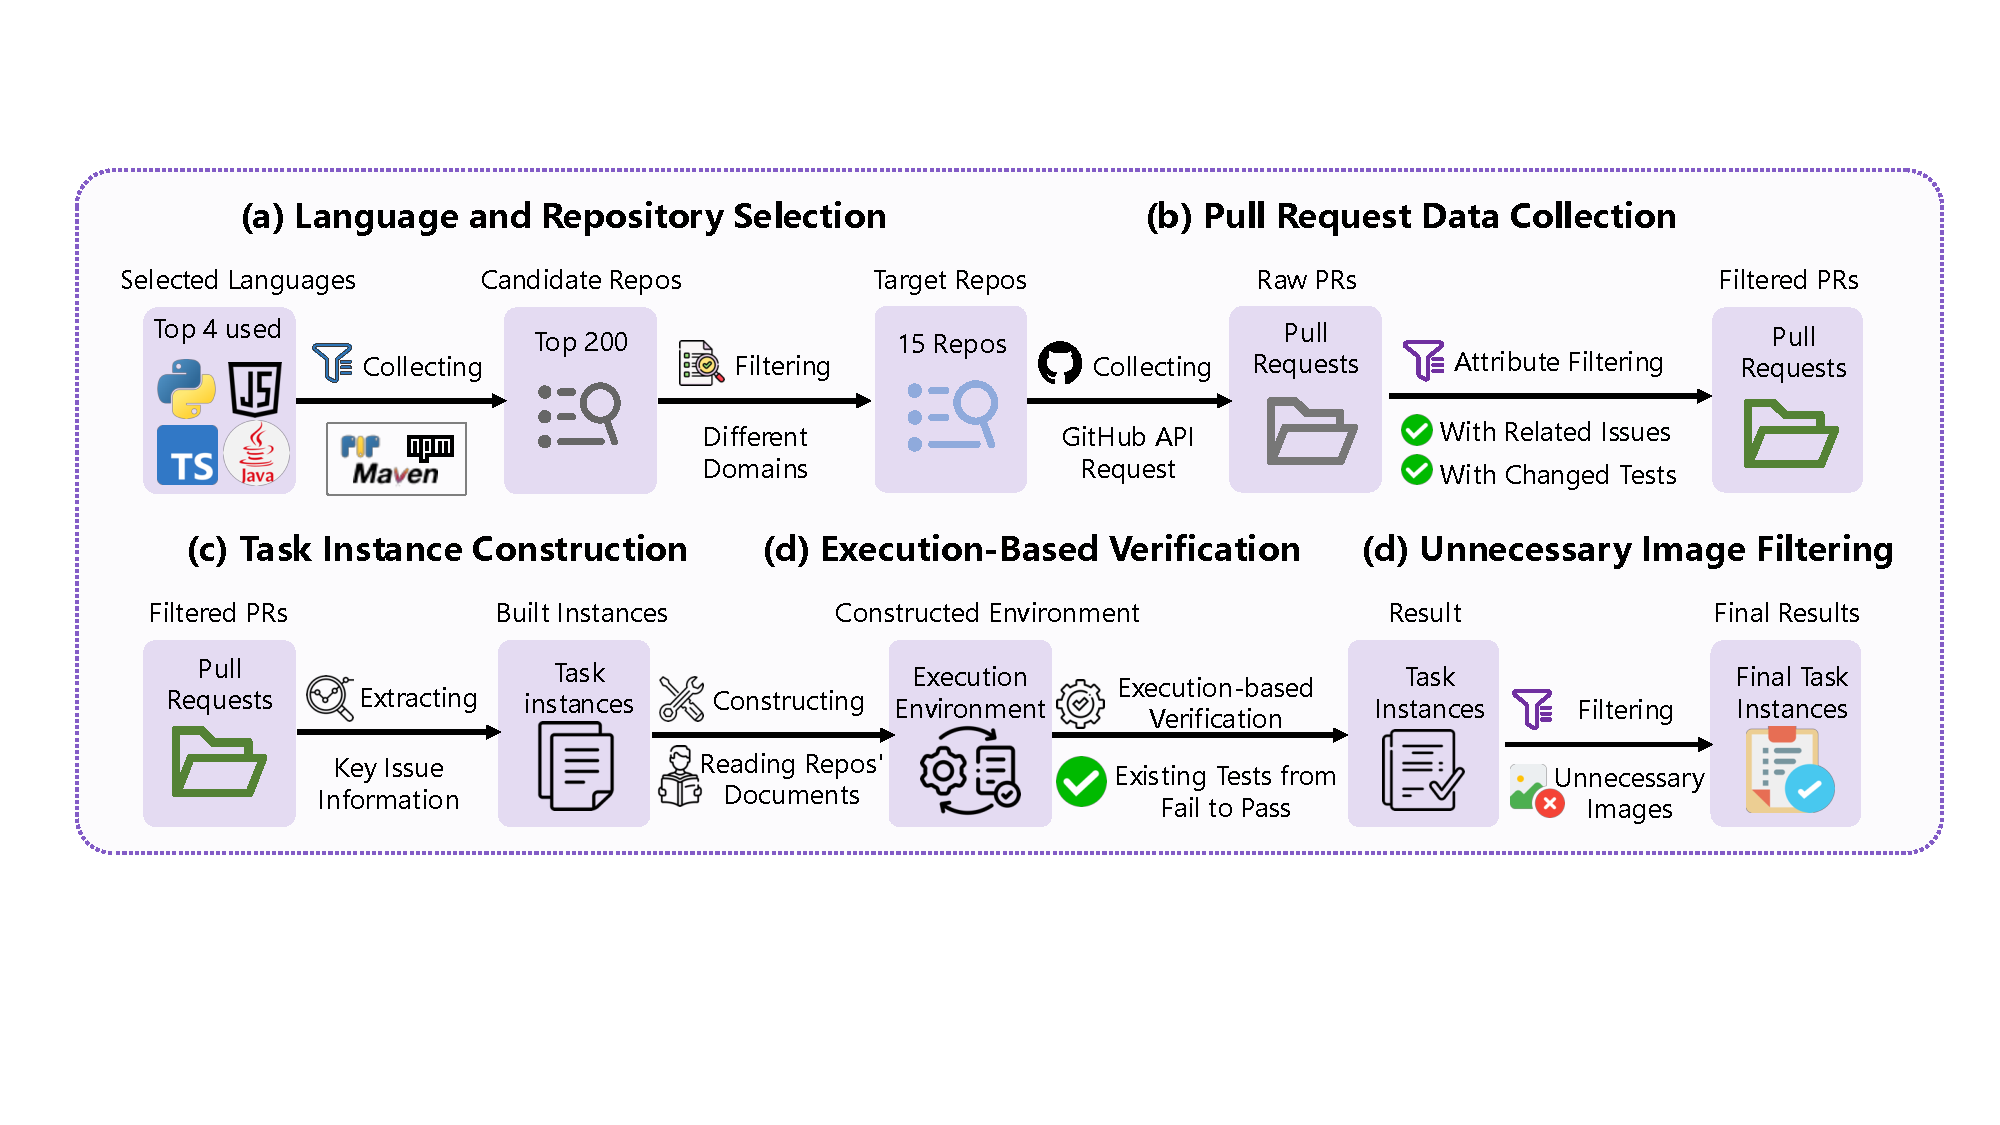
\includegraphics[width=\linewidth]{figures/BenchmarkConstructionV7.pdf}
    % \vspace{-1em}
    \figmargin
    \caption{Overview of benchmark construction.}
   % \vspace{-0.5em}
    \label{fig:DataCollection}
\end{figure}

\subsection{Language and Repository Selection}

\subsubsection{Language Selection.} Before building our multilingual benchmark, we first select widely used programming languages as target languages. Based on the latest GitHub report,\footnote{\url{https://github.blog/news-insights/research/the-state-of-open-source-and-ai/}} JavaScript, Python, TypeScript, and Java are among the most popular languages, reflecting their extensive use in the developer community. Besides, these languages are widely used in different domains: Python is common in AI and data science, JavaScript and TypeScript are crucial for web development, and Java is widely applied in large-scale systems and backend development. Considering the popularity and significance of these languages, we choose them as our target languages.

\subsubsection{Repository Selection.} 

To ensure the popularity of the target repositories, we use the download counts from language-specific package management tools. For Python, we select repositories based on pip download counts. For Java, we use Maven, and for JavaScript and TypeScript, we rely on npm. For each language, we select the top 200 repositories with the highest download counts. Next, using the GitHub API~\cite{github-rest-api}, we collect the tags from these repositories. Based on the tags, we select 15 popular repositories from different domains as our target repositories. This approach ensures that our selection covers diverse fields and focuses on highly used repositories.

\subsection{Pull Request Data Collection} 
\subsubsection{Collection of Pull Requests.} In GitHub repositories, developers submit pull requests to report potential issues and resolve existing issues. In this stage, we use the GitHub Developer API~\cite{github-rest-api} to collect pull requests from each repository. We then retain only those pull requests in the merged state. This is because merged pull requests have been generally reviewed by the repository maintainers and successfully integrated into the codebase. Additionally, we set a cutoff date of July 31, 2024, and only keep pull requests that were merged before this date, using this as a starting point for future data collection.

% This process guarantees the correctness and quality of the pull requests. 

% Repository-level code translation aims to translate the entire repository from one language to another. Due to the limited context window and performance of non-LLM techniques~\cite{pan2024lost}, we use LLMs to achieve the translation tasks.

% \subsubsection{Language Selection}
% Referring to the \texttt{TIOBE index}~\cite{TIOBE-Index} for language popularity, we select Python, C++, Java, C, and C\# as candidate languages. Considering Python is popular for its simplicity, ease of use, and rapid prototyping, but has low execution efficiency, while Java, on the other hand, is favored for enterprise-level applications, offering better performance, stability, and faster execution~\cite{szafraniec2022code}, we choose Python as the source language and Java as the target language. 

\subsubsection{Attribute-Based Filtering.}
To make that each collected data contains issue descriptions and tests to verify the correctness of submitted solutions, following the approach of SWE-bench~\cite{jimenez2023swe}, we use the attribute-based filtering method to filter the collected pull requests data further:

\begin{itemize}[left=10pt]
    \item \textbf{Keep PRs resolving at least one issue.} In the GitHub repository, when submitting a pull request that resolves some issues, the developer uses statements like ``fix \#403'' in the title or body to indicate which issues are resolved. Following the implementation code of SWE-bench,\footnote{\url{https://github.com/princeton-nlp/SWE-bench/blob/main/swebench/collect/utils.py}} we first gather all text content from the title, body, and commit messages of each pull request. We then extract each issue number (e.g., ``\#403'') from this aggregated content using regular expressions. Finally, we filter out pull request data without any relevant issue number.
    \item \textbf{Keep PRs with test files changed.}
When fixing a bug or adding a new feature, developers often submit a pull request containing code changes in test files. These test files offer a great solution to verify whether the bug is fixed or the feature is implemented successfully. Following SWE-bench,$^4$ we first identify test files in the changed files of a pull request by checking if their full paths contain keywords like ``test'' or ``testing''. Then, we filter out pull request data without any test file changed.
% only when the full path of a file in the pull request contains keywords like ``test'' or ``testing'', we consider this file as test files. The pull request without any test file is filtered. 
\end{itemize}

\begin{figure}
    \centering
    % \vspace{-10pt}
    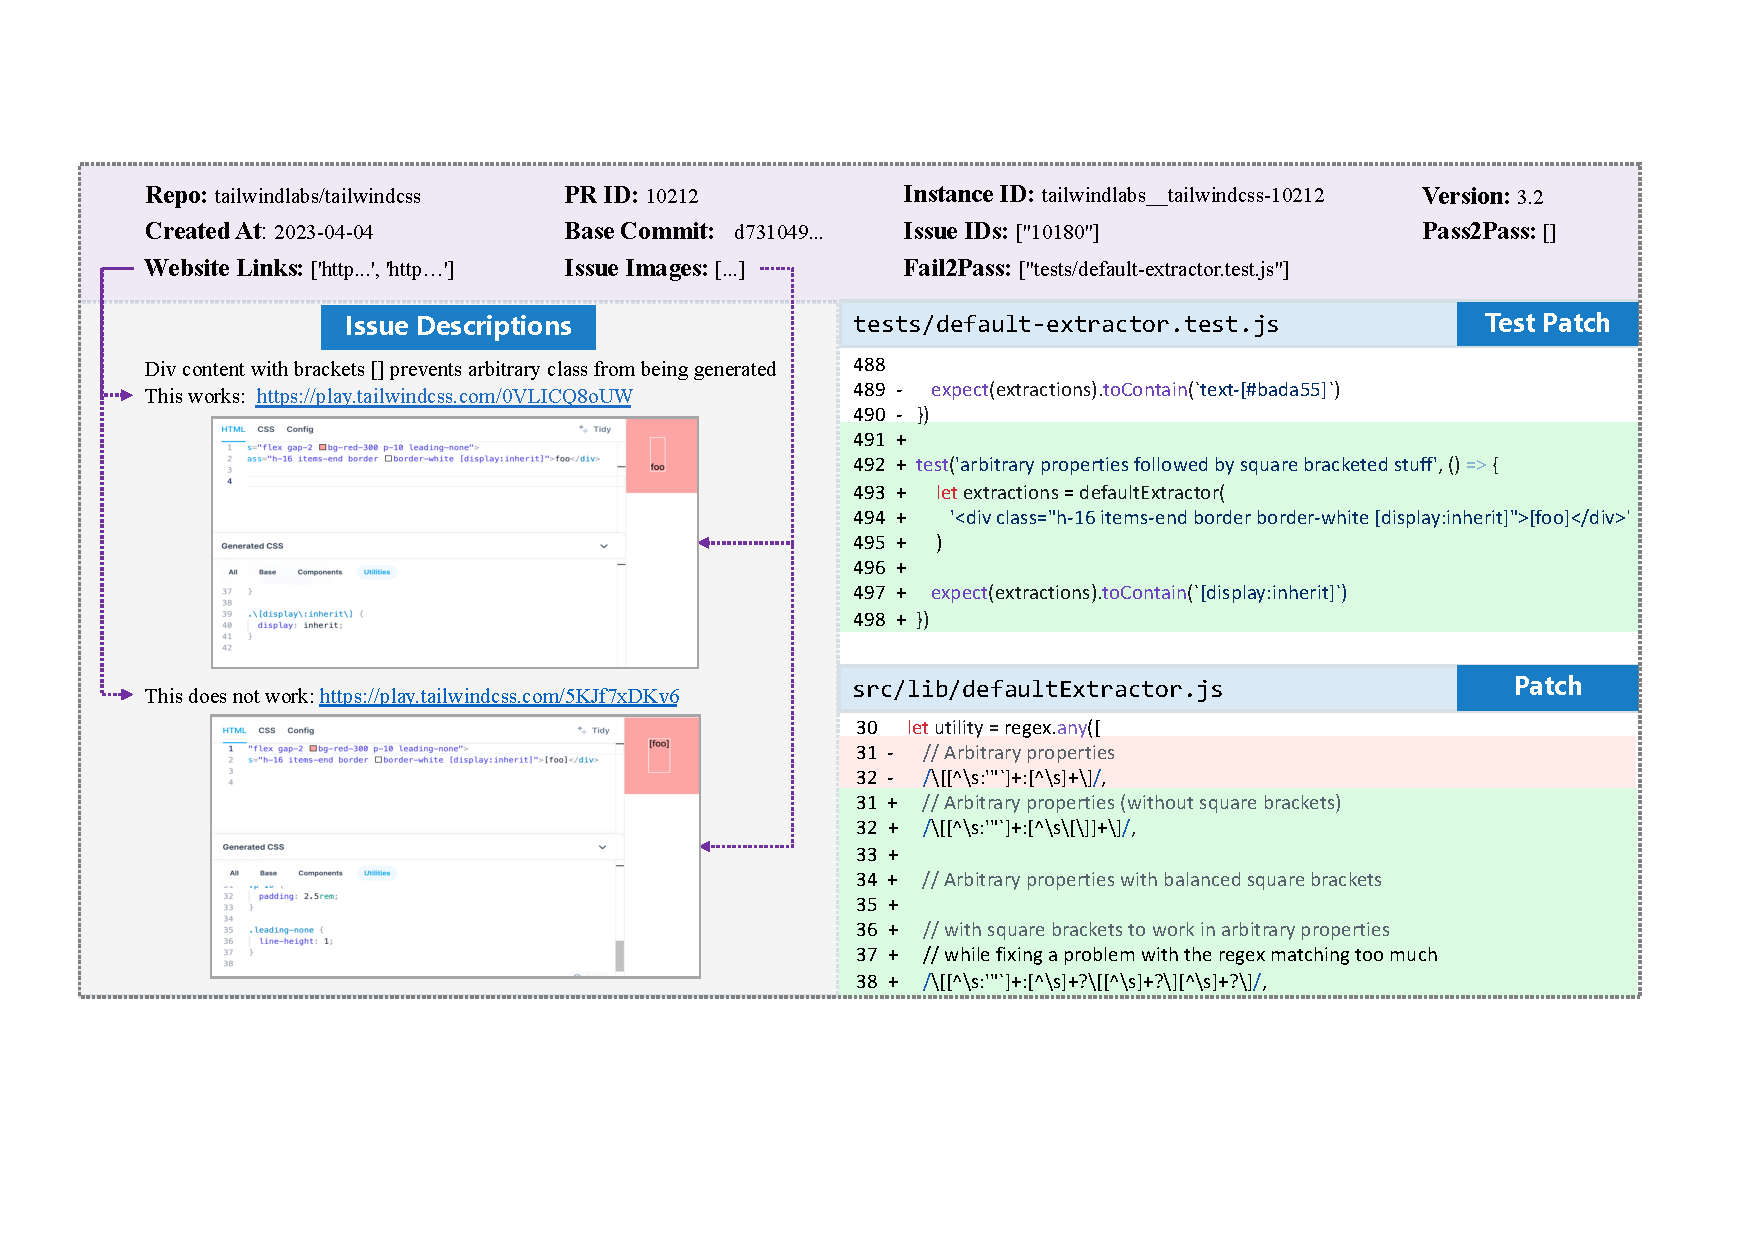
\includegraphics[width=\linewidth]{figures/TaskInstanceExampleV4.pdf}
    % \vspace{-1em}
    \figmargin
    \caption{An example of task instance \texttt{tailwindlabs__tailwindcss-10212}.} %Detailed information about the task instance tailwindlabs__tailwindcss-10212.}
    % 
   % \vspace{-0.5em}
    \label{fig:TaskInstanceExample}
\end{figure}
% \footnote{\url{https://github.com/tailwindlabs/tailwindcss/issues/10180}}

\subsection{Task Instance Construction}
After collecting raw data of pull requests, we build task instances using GitHub Developer API~\cite{github-rest-api} to obtain key information from each pull request. An example of a task instance is shown in Figure~\ref{fig:TaskInstanceExample}. Here, we introduce the attributes of this task instance:

\begin{itemize}[left=10pt]
    \item \textbf{Repo.} This attribute refers to which repository the task instance belongs to. In Figure~\ref{fig:TaskInstanceExample}, this instance is from the repository ``tailwindlabs/tailwindcss''. 
    \item \textbf{PR ID.} This attribute refers to which pull request the task instance belongs to. Each pull request has a unique ID, such as 10212.
    \item  \textbf{Instance ID.} This attribute is a unique identifier for the task instance, composed of ``Repo'' and ``PR ID''. For example, the ``tailwindlabs\_\_tailwindcss-10943'' means this task instance is obtained from pull \#10943 in the repository ``tailwindlabs/tailwindcss''.
    \item  \textbf{Created At.} This attribute refers to the date when the pull request was created.
    \item \textbf{Issue IDs.} This attribute refers to the ID numbers of the issues that are resolved by the pull request. For example, the issue number of instance ``tailwindlabs\_\_tailwindcss-10943'' is 10937, which means this pull request resolves the issue \#10937.
    \item \textbf{Issue Descriptions.} This attribute refers to the text descriptions of issues related to the task instance. For example, as shown in Figure~\ref{fig:TaskInstanceExample}, the problem statement describes unexpected results of running programs. In the evaluation, this problem statement serves as the input of the task instance. Following the approach of  SWE-bench, we extract and concatenate the issue's title and body to form the content of the problem statement.
    \item \textbf{Issue Images.} This attribute refers to images in issue descriptions.  As shown in Figure~\ref{fig:TaskInstanceExample}, this user attaches two images to describe the unexpected results of running programs. In the evaluation, these images can provide visual information for resolving issues. Since GitHub uses URLs to display images, we extract URLs containing ``png'' or ``jpg'' from the issue body of task instances. We then manually check whether these images are relevant to the content of the issue. Because not all task instances include images, this is an optional attribute.
    \item \textbf{Website Links.} This attribute refers to some website links users share to help describe reported issues. As shown in Figure~\ref{fig:TaskInstanceExample}, this user shares two links to an online code execution platform, where the reproduced code and execution results are presented. These links provide execution environments for developers to understand issues by debugging.  We manually check website links in each issue and keep website links that are crucial for resolving this issue. This is an optional attribute because not all task instances include such links. 

% additional context and valuable information for developers.
    % Some issue descriptions may contain important website links. 
% Sometimes, users use images to help describe the reported issue.
    
    \item \textbf{Version.} This attribute refers to the version of the repository when the pull request was created. Since different versions of the code repository may require different environment setups, this information helps construct the appropriate code environment for each task instance. Considering that version information is typically updated in configuration files, we locate the configuration file corresponding to each task instance and extract the version information. For example, Python versions are usually stored in the \texttt{setup.py} file, JavaScript and TypeScript versions in \texttt{package.json}, and Java versions in \texttt{pom.xml}.
    \item \textbf{Base Commit.} This attribute is a unique commit ID that the original pull request is based on. Using the base\_commit, we can revert the GitHub repository to the state before the pull request was applied. This helps us construct the correct code repository environment for the target issues. We extract this information using the GitHub Developer API~\cite{github-rest-api}.
      \item \textbf{Test Patch.} This attribute refers to the code changes in the pull request that are used to test the modified source code. In the evaluation, this content is used to run tests to verify the correctness of the submitted solution. Following the approach of SWE-bench~\cite{jimenez2023swe}, we check the file paths of each hunk in the code changes and retain only those where the file path contains keywords like ``test'' or ``testing.'' Additionally, for Java, we consider any Java file where the file name starts or ends with ``Test'' (e.g., \texttt{TestClass.java} or \texttt{MyClassTest.java)} as part of the test patch.
    \item \textbf{Patch.} This attribute refers to the code changes in the pull request that specifically address resolving the issue. This content provides the ground truth solution for the issue. To collect this data, we first examine each hunk in the code changes and filter out hunks related to testing. Then, we use the Python library Pygments~\cite{pygments} to check the file paths in each hunk and determine if they belong to the source files of the target programming language. For example, in Python repositories, files ending in ``.py'' are recognized as Python source files. This helps us exclude irrelevant files, such as documentation files ending in ``.md''. Additionally, we collect certain configuration files that are crucial for the patch’s correctness. For instance, for JavaScript, we gather changes in \texttt{package.json}, and for Java, we include changes in \texttt{pom.xml}. These specific changes are important for ensuring the patch's correctness.
    
    \item \textbf{FAIL2PASS.} This attribute refers to tests or test cases that are changed from ``fail'' status to ``pass'' status after applying the gold patch. These tests or test cases are used to verify whether the submitted solution can resolve issues in the task instance.
    \item \textbf{PASS2PASS.} This attribute refers to tests or test cases that maintain a ``pass'' status both before and after applying the gold patch. This attribute can be used to verify whether the submitted solution does not change the function of the original source code. 
\end{itemize}

% This attribute refers to the code changes in the pull request that are used to test the modified source code. In the evaluation, this content is used to run tests to verify the correctness of the submitted solution.

\subsection{Execution-Based Verification} 
In this section,  we conduct execution-based verification to make each task instance have paired tests to check the correctness of submitted solutions. First, we construct an execution environment for each task instance and verify its correctness. Second, following the approach of SWE-bench~\cite{jimenez2023swe}, we conduct execution-based filtering to filter task instances without FAIL2PASS tests or test cases. The remaining task instances are considered valid data on \Swebenchx.

% To ensure that each collected task instance can be verified by running paired tests, following the SWE-bench, we conduct execution-based verification for each candidates. Firstly, we attempt to build execution environment for each task instance. And then we run tests 

\subsubsection{Environment Construction.} 
Before conducting execution-based filtering, we create an isolated execution environment for each task instance using Docker~\cite{docker} to minimize potential conflicts across environments. For each task instance, we define all setup commands in a \texttt{Dockerfile} and bash scripts, which are then executed to set up the Docker environment for each instance.



The execution environment includes the codebase before the issue was resolved and its required dependencies. For each task instance, we first use \texttt{Git}~\cite{git} to clone the repository. Then, with the task instance's ``Base Commit'' attribute, we use \texttt{Git} to revert the repository to the state before the pull request addressing the issue was submitted. To set up the correct dependencies, we refer to development documentation in the codebase, such as \texttt{README.md} and \texttt{CONTRIBUTING.md}, which often provide guidance on how to build dependencies. Following these instructions, we install the necessary dependencies for the codebase. The process described above is written into the \texttt{Dockerfile} and bash scripts to automate the construction of the docker environment.

% Before conducting the execution-based filtering, we build an execution environment for each task instance. We utilize Docker to build isolated environment to reduce potential conflicts among different environments. For each task instance, all environment setup commands are written in \texttt{Dockerfile} and bash scripts.

% using  reducing potential conflicts. We construct the environment by writing a Dockerfile and running setup scripts within the container. We find that some documentation in the codebase such as \texttt{README.MD} and \texttt{CONTRIBUTING.MD}, can provide useful guidance on how to set up correct dependencies.

% Building environments for task instances is challenging due to complex dependencies. We find that some documentation in a repository such as \texttt{README.MD} and \texttt{CONTRIBUTING.MD}, can provide useful guidance on how to set up a correct code environment. First, we switch the repository to the version matching the task instance, then follow these files to identify the necessary setup commands, including installing dependencies, configuring services, and setting environment variables, etc. 

%考虑到版本...
% \subsubsection{Test Command Generation}
\subsubsection{Environment Verification.}After building the execution environment successfully, we need to verify its correctness. In this step, our aim is to ensure that all tests in the test patch can be passed after applying the gold patch to the environment. Firstly, we update test files by applying the test patch to the codebase. Then, we apply the gold patch to the codebase and run relevant tests to obtain test results. We consider the constructed environment successfully verified only if all test cases pass. Otherwise, we think this environment needs further improvements.
\subsubsection{Execution-Based Filtering}
After building the execution environment, the next step is to verify if the tests can effectively evaluate the correctness of the submitted patch. Ideally, after applying the solution (gold patch), we expect the status of certain test cases to change from ``fail'' to ``pass'', indicating that the solution has addressed specific issues. We refer to these as FAIL2PASS test cases, which serve to verify that the patch has resolved the intended issue in the task instance. Test cases that maintain a 'pass' status throughout this process are called PASS2PASS test cases. These help ensure that the submitted patch does not change the original functionality of the code.

Following the approach of SWE-bench~\cite{jimenez2023swe}, we first run the relevant tests before and after applying the gold patch to observe whether there exist FAIL2PASS test cases. Then, We only retain task instances that contain at least one FAIL2PASS test case. Finally, we manually check whether the FAIL2PASS test cases match the tests  added or modified in the test patch, ensuring higher reliability in our evaluation process.


\subsection{Unnecessary Image Filtering}  
After building task instances, we manually check images in each task instance to determine whether these images are essential for resolving issues. For example, while some users utilize screenshots of error messages to describe issues, these error messages may already be included in the text of the issue descriptions. In such cases, we filter these unnecessary images, as they do not provide crucial information for resolving issues.
The results of the filtering process are presented in Table~\ref{table:filteringProcess}. Before filtering, the dataset contains 39 task instances with an average of 1.7 images per instance, covering ten repositories across all four languages. After filtering out unnecessary images, \Swebenchx remains 19 instances with an average of 1.8 images per instance, now covering seven repositories across three languages (e.g., Python, TypeScript, and JavaScript).

 % This initial filtering resulted in 42 instances. Next, we manually check whether the images are essential for resolving the issue. For example, if an image contains reproduction steps or code snippets that are already provided in the text, we exclude that instance, as the  After this review, we finally build SWE-bench-Visual, a subset containing 19 task instances that span three different programming languages. The statistics of SWE-bench-Visual are shown in Table~\ref{table:swebenchv}.

% When reporting issues on GitHub, users often include images in addition to textual descriptions to help illustrate the problem. Motivated by this, we constructed a subset of \Swebenchx focused on issues with visual input.

\begin{table}[t]
  \centering
  \footnotesize
  \setlength\tabcolsep{1.5pt}
  \caption{Results of filtering unnecessary images.}
  \label{table:filteringProcess}
  \tabmargin
  % \resizebox{\columnwidth}{!}{
    \begin{tabular}{ccccccc}
    \toprule
    \multirow{2}{*}{\textbf{Language}} & \multicolumn{3}{c}{\textbf{Before Filtering}} & \multicolumn{3}{c}{\textbf{After Filtering}} \\
    \cmidrule(r){2-4} \cmidrule(r){5-7}
    & \textbf{\# Instances} & \textbf{\# Avg Images} & \textbf{\# Repos} & \textbf{\# Instances} & \textbf{\# Avg Images} & \textbf{\# Repos} \\
    \midrule
    
    \textbf{All} & 39  & 1.7 & 10 &  19 & 1.8 & 7 \\
    \midrule
    \quad Python & 7 & 1.3 & 2 & 2 & 1.0 & 2 \\
    \quad TypeScript  & 15 & 1.7 & 2 & 12 & 1.9 & 2 \\
    \quad JavaScript  & 15 & 1.8 & 3 & 5 & 1.8 & 3 \\
    \quad Java  & 2 & 1.5 & 2 & 0 & 0.0 & 0 \\

    

    \bottomrule
    \end{tabular}
    % }%

\end{table}
\secmargin
\section{\Swebenchx}
\subsection{Statistics of \Swebenchx}
After constructing the benchmark, \Swebenchx includes 959 instances collected from 15 repositories, covering four programming languages: Python, JavaScript, TypeScript, and Java. The details of the repositories included in the dataset are presented in Table~\ref{table:statitics}, which lists the programming language used, the number of instances, and the license for each repository. The licenses ensure that our dataset can be freely accessed and used for research purposes.


\begin{table}[t]

\centering
\caption{Statistics of \Swebenchx repositories.}
\footnotesize
\tabmargin
\begin{tabular}{lccc}
\toprule
\textbf{Repository} & \textbf{\# Instances} & \textbf{\# Languages} & \textbf{License} \\
\midrule
python/mypy & 189 & Python & BSD 3-Clause \\
% \hline
pyca/cryptography & 21 & Python & BSD 3-Clause  \\
% \hline
dateutil/dateutil & 36 & Python & BSD 3-Clause \\
% \hline
tqdm/tqdm & 23 & Python & MIT \\
% \hline
statsmodels/statsmodels & 76 & Python & BSD 3-Clause \\
% \hline
redis/redis-py & 29 & Python & MIT \\
% \hline
iamkun/dayjs & 93 & JavaScript & MIT \\
% \hline
prettier/prettier & 119 & JavaScript & MIT \\
% \hline
webpack/webpack & 58 & JavaScript & MIT \\
% \hline
jestjs/jest & 31 & TypeScript & MIT \\
% \hline
babel/babel & 79 & TypeScript & MIT \\
% \hline
tailwindlabs/tailwindcss & 100 & TypeScript & MIT \\
% \hline
netty/netty & 54 & Java & Apache-2.0 \\
% \hline
google/gson & 21 & Java & Apache-2.0 \\
% \hline
assertj/assertj & 30 & Java & Apache-2.0 \\
% \hline
\toprule
\end{tabular}

\label{table:statitics}
\end{table}

We also analyze the characteristics of task instances, as summarized in Table~\ref{table:dataAnalysis}. We can find that task instances contain a long issue text, including 194 words on average. The codebase includes 995 files and 257K lines of code on average, showing the complexity of the codebase. Besides, the gold patches require modifications across 46 lines, 2.2 functions, and 1.2 files on average. These characteristics highlight the complexity of GitHub issue resolution tasks.
% we can also find the ground truth of instances need to edit many code lines, functions and files, and lots of tests need to run for verification. These characteristics highlight the complexity of GitHub issue resolution tasks.
% is large and includes lots of files and code lines.

\begin{table}[t]
\caption{Data analysis for our benchmark.} 
\label{table:dataAnalysis}
\tabmargin
\centering
\footnotesize
\begin{tabular}{cccc}
\toprule%第一道横线
& &Mean&Max \\
\midrule
Issue Text&Length (Words)&194&1,685 \\
\midrule
\multirow{2}{*}{Codebase}&\# Files (non-test)&995&3,016 \\%Data1跨两行，自动表格宽度
&\# Lines (non-test)&257K&1,010K \\
\midrule
\multirow{3}{*}{Gold Patch}&\# Lines edited& 46.3 & 1,657\\%Data1跨两行，自动表格宽度
&\# Files edited&1.2&30 \\
&\# Func. edited&2.2&131 \\
\midrule
\multirow{2}{*}{Tests}&\# Fail to Pass&3.3&1,056 \\%Data1跨两行，自动表格宽度
&\# Total&135.1&4,820 \\
\bottomrule
\end{tabular}
\end{table}

% 193.7


\subsection{Diversity of \Swebenchx}  
In this section, we introduce the diversity of \Swebenchx from three aspects: diversity of programming languages, diversity of repository domains, and diverse modality of input information. 


\subsubsection{Diversity of Programming Languages}

Our dataset contains issues from repositories in four widely used programming languages: Python, Java, JavaScript, and TypeScript. Python is known for its readability and extensive library support and is widely used in data science and machine learning. Java is commonly used in large-scale applications due to its great performance and robustness. JavaScript dominates web development with its dynamic capabilities. TypeScript is a statically typed superset of JavaScript, which adds type safety to JavaScript's flexibility.
Resolving issues from repositories across different programming languages requires distinct background knowledge. For each issue, we use its gold patch as a reference to analyze the required background knowledge. Each label of background knowledge can be found in developer documentation of these four languages~\cite{jsDocs,tsDocs,javaDocs,pythonDocs}. The analysis results are shown in Table~\ref{table:languageFeatures}. For example, we find issues in the JavaScript repository require background knowledge of both JavaScript and TypeScript (e.g., ``Arrow Functions'' and ``interface''). By identifying this rich background knowledge, our dataset enables researchers to design issue resolution methods applicable across different programming languages.
% By identifying the specific background knowledge necessary for each language, future researchers can design more generalizable algorithms that leverage the nuances of different programming languages in issue resolution.

\begin{table}[t]
\scriptsize
\centering
\caption{Categories of background knowledge in different programming languages contained in gold patch.}
\label{table:languageFeatures}
\tabmargin
\begin{tabular}{c l}
\toprule
    \bf{Language of Repository}  & \bf{Background Knowledge Contained in Gold Patch} \\
\midrule
    Python  & ``Decorator''; ``Generator''; ``Iterator''; ``Reflection''; ``Wraps''\\
    JavaScript & ``Anonymous Functions''; ``Arrow Functions''; ``Event-driven''; ``Interface''; \\
    TypeScript  & ``Anonymous Functions''; ``Arrow Functions''; ``Enum''; ``Generics''; ``Interface''; ``Type Aliases'';  \\
    Java  & ``Abstract Classes''; ``Annotations''; ``Generics''; ``Inheritance''; ``Interface'';  ``Reflection'';  \\
    % JavaScript & "Arrow Functions": 46; "Anonymous Functions": 5; "Event-driven": 25; "Interface":31; \\
    % TypeScript  & "Interface":20;"Type Aliases":32;"Enums”;"Generics";\\
    % Java  & "Inheritance": 14; "Interface": 14; "Generics": 28; "Reflection"; "Abstract Classes"; "Annotations"; \\
\bottomrule
\end{tabular}

\end{table}

\subsubsection{Diversity of Repository Domains.} In this section, we present the diverse range of domains covered by the repositories included in our benchmark. We first collect a brief introduction from the GitHub summary of each repository and label them with relevant domain tags. As shown in Table~\ref{table:repoSummary}, our benchmark covers domains as follow:

\begin{itemize}[left=10pt]

\item \textbf{Code quality (35.2\%).} Code quality tool is widely used to help developers improve code readability and maintainability. For instance, ``Prettier'' automatically formats code to ensure consistent style, making it more readable and maintainable.
% For example, developer can use ``mypy'' to check type in Python

\item \textbf{Web development (24.7\%).}  
Web development tools like ``tailwindcss'' are widely used for building modern, responsive user interfaces, facilitating efficient web development and ensuring compatibility with modern browsers and frameworks.

\item \textbf{Time tools (13.5\%).}  
Repositories such as ``dateutil'' provide crucial utilities for handling time and date operations. These libraries are widely used in various applications, particularly in scheduling and time-sensitive tasks across industries.

\item \textbf{Network tools (8.7\%).}  
Repositories like ``redis-py'' provide fundamental tools for managing databases and building scalable network applications. These libraries are key to developing high-performance, distributed systems.

\item \textbf{Statistical modeling (7.9\%).}  The ``statsmodels'' library provides rich statistical and econometric tools essential for data-driven decision-making and financial trend modeling. Maintaining this repository requires rich knowledge of statistics and econometrics.

% The ``statsmodels'' library is widely used in fields like finance, where robust statistical analysis and econometrics are required for making data-driven decisions and modeling financial trends.

\item \textbf{Developer utility (4.4\%).}  
Developer Utility provides tools to enhance development productivity. For instance, ``gson'' simplifies JSON parsing and serialization in Java, while ``tqdm'' offers progress bars for Python, helping developers efficiently monitor and manage tasks.

\item \textbf{Test tool (3.2\%).}  
Test tools such as ``jest'' automate software testing, ensuring code correctness, reliability, and performance by detecting bugs and verifying expected functionality.

\item \textbf{Cryptography (2.4\%).}  
The ``cryptography'' repository offers essential cryptographic primitives and recipes, playing a critical role in securing communications and data, especially in sensitive fields like cybersecurity and financial services.

\end{itemize}

\begin{table}[t]
\centering
\footnotesize
\caption{Repository summary and domain tags.}
\tabmargin
\resizebox{\textwidth}{!}{%
% \begin{tabular}{llll} & \textbf{Percentage} & 35.2\% (338/959) 35.2\% (338/959) 35.2\% (338/959)
\begin{tabular}{lll}
\toprule
\textbf{Repository} & \textbf{Summary} & \textbf{Domain Tag} \\
\midrule
python/mypy & Optional static typing for Python  & Code quality \\
prettier/prettier & Opinionated code formatter for JavaScript & Code quality \\
assertj/assertj & Library providing typed assertions for Java & Code quality \\
webpack/webpack & A bundler for javascript to pack modules & Web development\\
babel/babel & Compiler for writing next generation JavaScript. & Web development\\
tailwindlabs/tailwindcss & Utility-first CSS framework for UI development & Web development\\
dateutil/dateutil & Extensions to the standard Python datetime features & Time tool\\
iamkun/dayjs & Lightweight immutable date-time library & Time tool\\
redis/redis-py & Redis python client & Network tool\\
netty/netty & Asynchronous network application framework & Network tool\\
statsmodels/statsmodels & Statistical modeling and econometrics in Python & Statitics modeling\\
tqdm/tqdm & Fast, Extensible Progress Bar for Python and CLI & Developer utility\\
google/gson & Java library for JSON serialization and deserialization &Developer utility\\
jestjs/jest & Testing Framework for JavaScript & Test tool\\
pyca/cryptography & Cryptographic recipes and primitives for Python & Cryptography\\

\toprule
\end{tabular}%
}

\label{table:repoSummary}
\end{table}

 % In SWE-bench, task inputs are provided solely in text format. However, on GitHub, users describe issues using a wider range of information types. 

% Text is the most common form of input in issue description, typically including reproduced code, error messages, environment configurations, etc. This type of information is well-suited for  LLMs to understand and process, making it an effective input for evaluating model capabilities.

\subsubsection{Diversity of Input Information Modalities} Previous benchmarks only focus on text information in issue descriptions, overlooking diverse multimodal information on issues. By manually reviewing issues in our benchmark, we identify three modalities of input: text information, image information, and website information.

 
\textbf{Textual information.} Text is the most common modality in GitHub issues, where users typically describe issues with details such as environment setup, reproduction code, error messages, etc.

\textbf{Image information.}
In addition to textual information, users often upload images to provide key details of reported issues. After analyzing images contained on \Swebenchx, we classify them into three types based on their purpose, as shown in Figure~\ref{fig:ImageExample}: 

\begin{itemize}[left=10pt]
    \item \textbf{Screenshots of reproduced code.}  Some users prefer to attach screenshots to demonstrate the code that reproduces an issue, as shown in Figure~\ref{fig:ImageExample} (a). 
    % Users often upload screenshots of their code to demonstrate how to reproduce the issue. This method is convenient for users, allowing them to bypass the need for text input. For example, in Figure~\ref{fig:ImageExample} (a), we see the user paste a screenshot to show the code that caused the issue.
 
    
    \item \textbf{Error messages or logs.}  Some users prefer taking screenshots of error messages or logs instead of copying the text, especially when the error is long or has complex formatting. In Figure~\ref{fig:ImageExample} (b), the user uploads a screenshot to show the error messages.
    
% Some users prefer to take screenshots of error messages or logs rather than copying the text. This is particularly common when error information is lengthy or formatted in a way that is easier to capture visually. In Figure~\ref{fig:ImageExample} (b), the user upload a screenshot of the error message to describe the issue.

% hese images are used to report unexpected results or behaviors of the code. understanding of how the code behaves incorrectly
    
    \item \textbf{Unexpected output or behavior of code.} These images are used to report unexpected results or behaviors after running the program.
    Unlike the previous two categories, these images often cannot be easily converted to text and require LLMs to understand the semantics of images with visual ability. For instance, in Figure~\ref{fig:ImageExample} (c), after updating the code version, the user noticed that the colors of the elements were incorrect. They used images to show the unexpected changes in the element colors. 
    % to explain the issue.

\end{itemize}
Image information presents new challenges for current LLMs, requiring models with visual abilities to understand images, extract key issue details, and ultimately assist in resolving issues.
% Issues including images require a multimodal language model capable of visual understanding to process them effectively. The model needs to correctly interpret the information in code screenshots, error messages, and the results displayed in images. This type of image-based information is useful for assessing an LLM's issue resolution capabilities in real software development scenarios.

\begin{figure}[t]
    \centering
    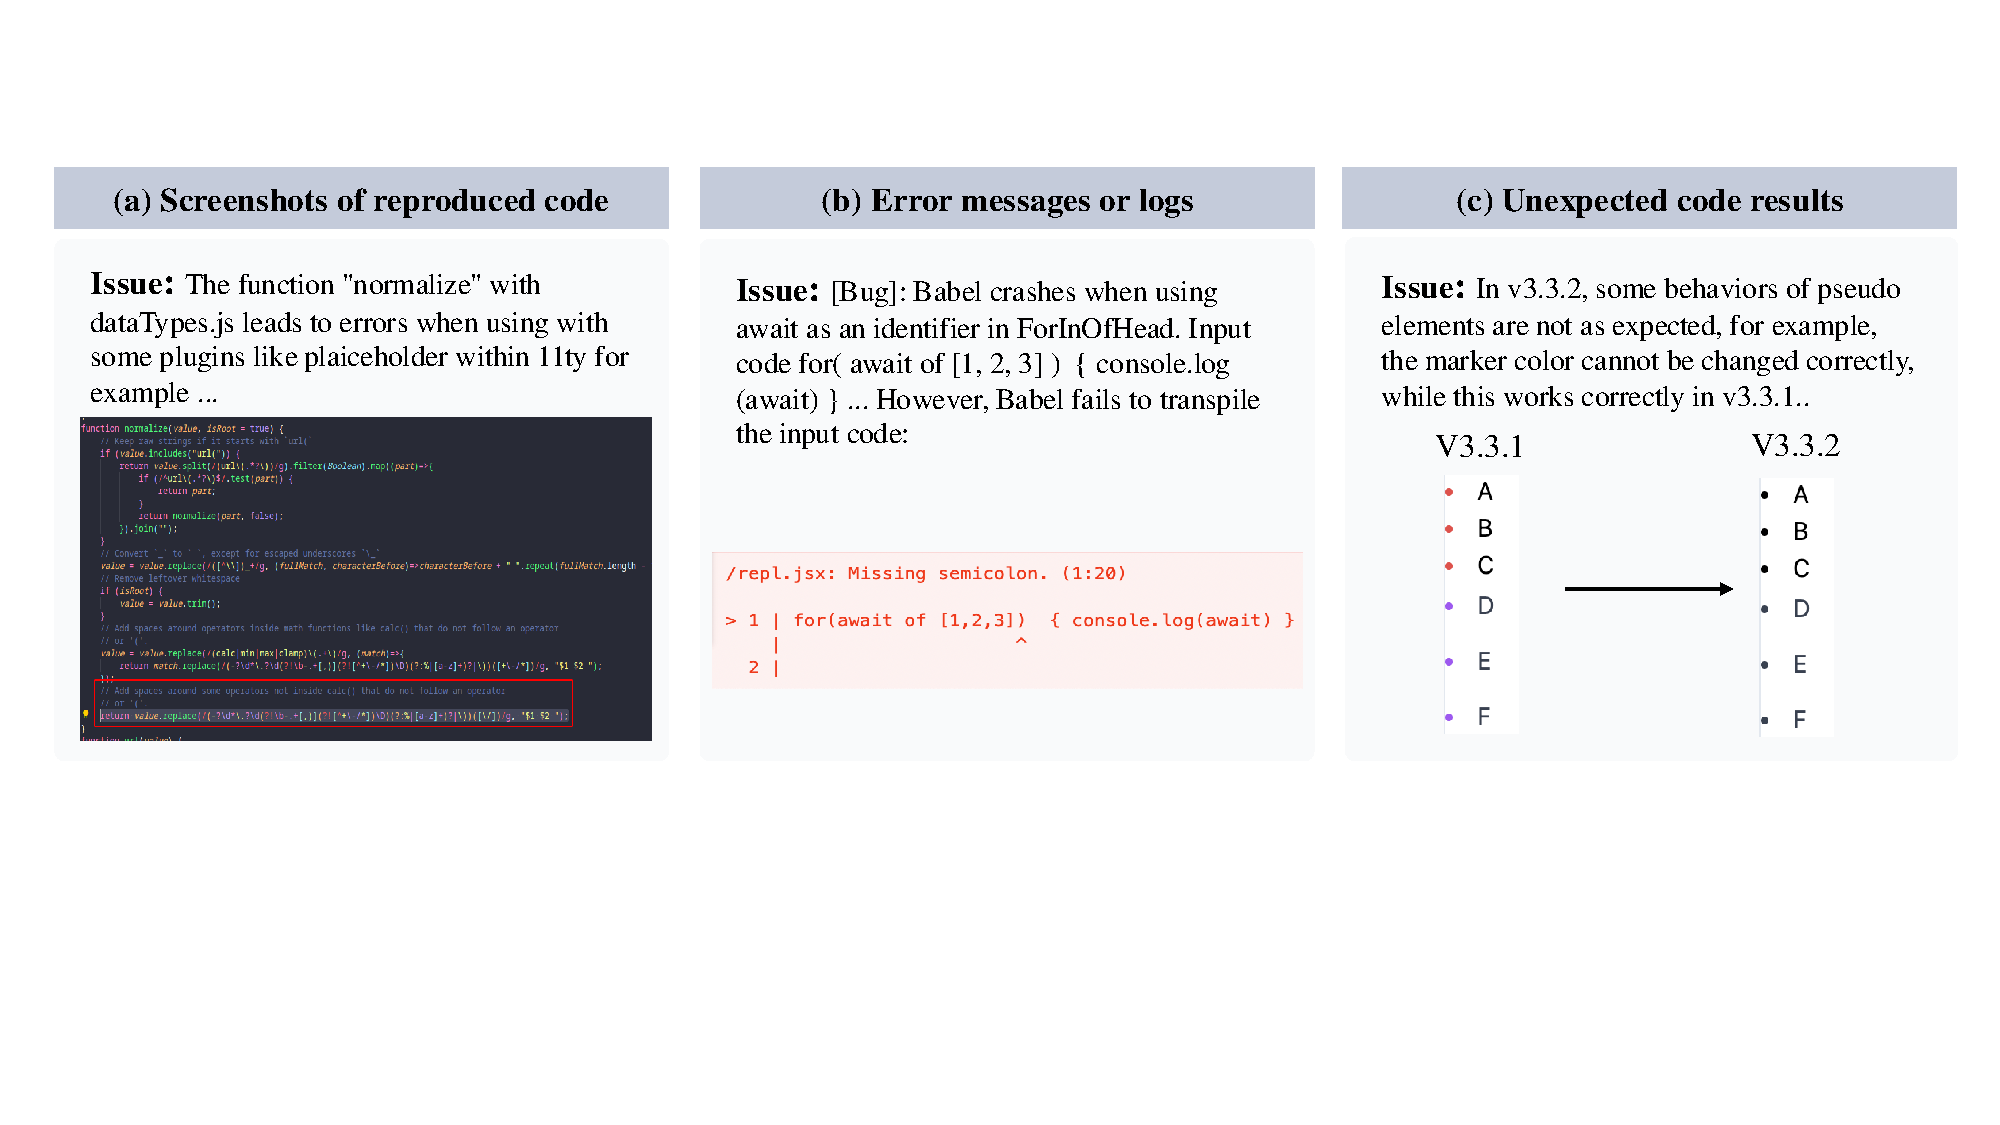
\includegraphics[width=\linewidth]{figures/ImageExampleV4.pdf}
    \figmargin
    \caption{Examples of images contained in issue descriptions.}
    \label{fig:ImageExample}
\end{figure}

% If this information is treated as plain text, it does not provide useful information for issues.

\textbf{Website information.} Website information refers to some website links that provide important details related to an issue.  For example, in the JavaScript and TypeScript GitHub communities, users often share links to online code execution platforms to help others reproduce reported issues. As shown in Figure~\ref{fig:url}, instead of providing the reproduced code directly, a user shares a link in the issue description that directs to ``Tailwind Play'', a website for debugging Tailwind CSS code online. These links allow developers to execute the reproduced code and observe errors in real-time. Unlike textual or image information, website information requires models to have web-browsing capabilities to interact with the website and obtain crucial information about issues.

% on these web pages may be in text format, it cannot be effectively processed if treated as plain text. 
% LLMs need web navigation capabilities to access these links and extract relevant information.
%

\begin{figure}[t]
    \centering
    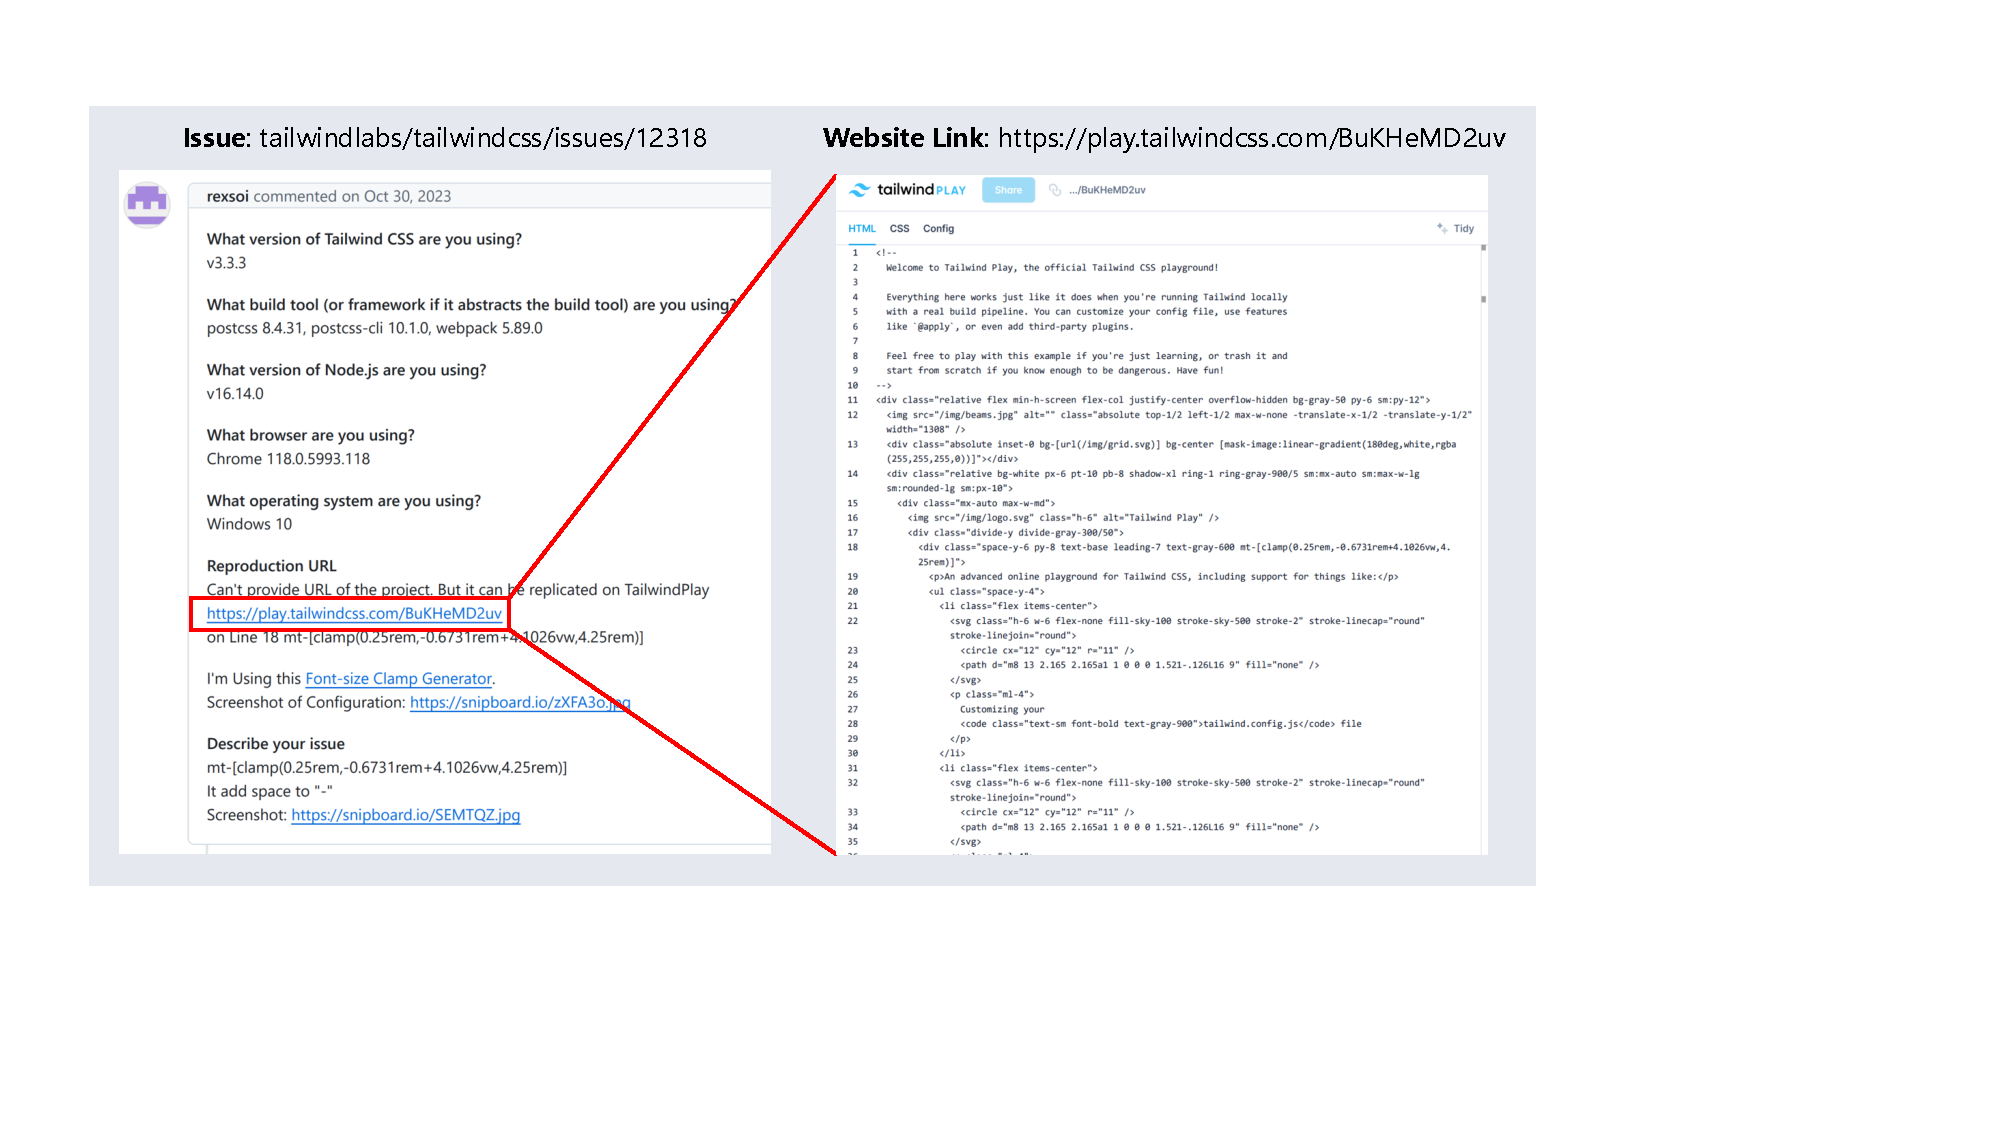
\includegraphics[width=\linewidth]{figures/WebsiteLinksV5.pdf}
    \figmargin
    \caption{An example of website links within an issue.}%\protect\footnotemark}
    \label{fig:url}
\end{figure}

% \begin{figure}[t]
%     \centering
%     % \vspace{-10pt}
%     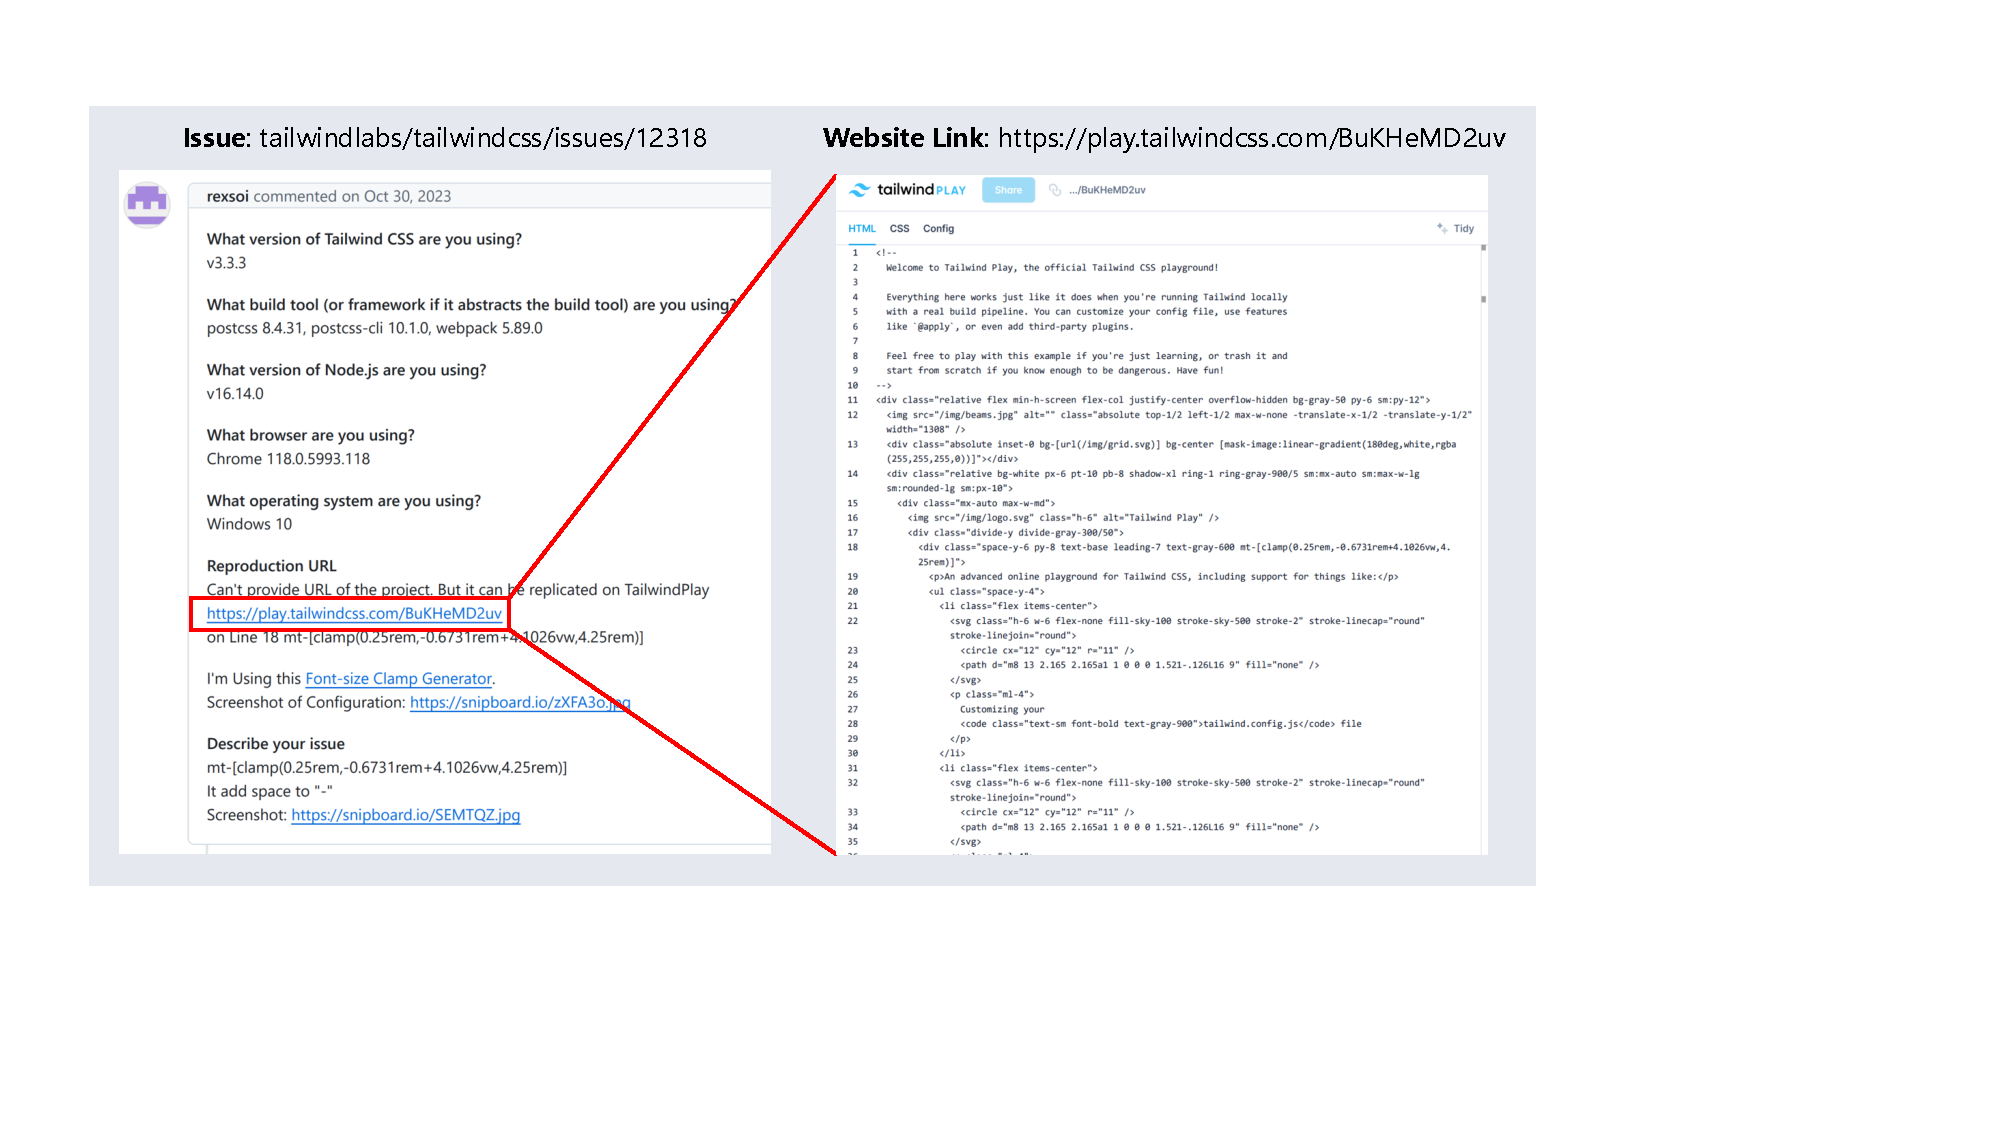
\includegraphics[width=\linewidth]{figures/WebsiteLinksV5.pdf}
%     % \vspace{-1em}
%     % \figmargin
%     \caption{An example of website links within an issue.\footnotemark}
%     \label{fig:url}
% \end{figure}

\footnotetext{\url{https://github.com/tailwindlabs/tailwindcss/issues/12318}}

\textbf{Distribution of different modality.} 
We analyze the modalities present in each issue to calculate their distribution. Our analysis shows that all issues include text information, with 31.0\% (297/959) also including website information, 4.1\% (39/959) containing image information, This distribution highlights the diversity of multimodal data on \Swebenchx.
%, offering a solid foundation for evaluating real-world issues. and 1.1\%(11/959) instances containing both image and website information. 
% We then investigate the distribution of various input types in our dataset. Given that a single issue may include multiple forms of input, such as text, images, or URLs, we classify the issues into four categories: text only, text + image, text + URL, and text + image + URL. We then categorize the dataset according to these types, and the results, as shown in Table~\ref{table:InputInfoTable}, reveal the prevalence of each input combination. \glh{still need revise..}Table~\ref{table:InputInfoTable} shows that while the majority of users (76.31\%) use text alone to describe issues, 19.16\% provide additional context with URLs, often linking to external resources for reproducing the problem. Additionally, 3.25\% of users incorporate images to visually demonstrate the issue, and 1.28\% combine all three types of information. These diverse inputs are crucial in issue resolution tasks, as images and URLs can provide valuable context that text alone cannot capture. To effectively resolve issues, it's important to consider how to fully utilize these rich inputs, integrating them into the issue resolution process to enhance accuracy and understanding. \glh{still need revise..}

% \begin{figure}[t]
%     \centering
%     % \vspace{-10pt}
%     
\includegraphics[width=0.6\linewidth]{ISSTA25-acmart-primary/figures/DistributionInputType.pdf}
%     % \vspace{-1em}
%     \caption{Distribution of different input information.}
%    % \vspace{-0.5em}
%     \label{fig:distribution}
% \end{figure}

% \begin{table}[t]
%   \centering
%   \footnotesize
%   \setlength\tabcolsep{1.5pt}
%    \caption{Distribution of different input information.\glh{to revise}} 
%   \label{table:InputInfoTable}
%   % \vspace*{-10pt}
%   % \resizebox{0.6\columnwidth}{!}{
%     \begin{tabular}{ccccc}
%     \hline
%     {\textbf{Input Infromation}} &{\textbf{Text Only}} &{\textbf{Text \& Weburls}} &{\textbf{Text \& Images}} &{\textbf{Text \& Weburls \& Images}} \\
%    \midrule
%     % Example Data
%        \textbf{Ratio} & 67.3\% & 28.7\% & 2.9\% & 1.1\%\\
%     % \GPT(vision)  & 4.2\% &45.8\%  & 0.072 & 8.3\% & 83.3\% &  \\
%     % \hline
     
%     \bottomrule
%     \end{tabular}
%     % }%

%   % \vspace*{-2em}
% \end{table}










% \begin{figure}[t]
%     \centering
%     % \vspace{-10pt}
%     
\includegraphics[width=0.7\linewidth]{ISSTA25-acmart-primary/figures/issueWithImage.jpg}
%     % \vspace{-1em}
%     \caption{Overview of the translation process.}
%    % \vspace{-0.5em}
%     \label{fig:issueWithImage}
% \end{figure}
\secmargin
\section{Evaluation}

In this section, we first evaluate the issue resolution ability of three advanced LLMs on \Swebenchx. We then  evaluate the performances of LLMs on issues requires image understanding. Finally, we investigate why LLMs fails to resolve issues on \Swebenchx. %We will first introduce the setup of our experiments. Then, 
We answer the following research questions: 
%\hy{the purpose of experiments and evaluation should be described at the beginning of the section. for example, evaluation the performance of recent LLMs on the proposed benchmark, etc}\glh{revised}

% In this section, to explore LLMs's performance on \Swebenchx:

% \hy{is it Experimental Results? can merge it with Section 6? also, say what the purpose of the evaluation is}\glh{revised}


%     \hy{this is what did for constructing the benchmark (your purpose/plan/motivation/design), why does it become a RQ?} \glh{Here we attempt to conduct some further analysis on our dataset to prove the diversity of our dataset. For example, we will analyze what knowledge are necessary for resolving issues in different languages manually. But i am not sure if this is appropriate. }\hy{i think it is not a RQ,it should be described in Section 5. The purpose of the evaluation should be made clearer} \glh{revised}

\begin{itemize}
    % \item \textbf{RQ1:} How diverse is the \Swebenchx? 

    \item \textbf{RQ1:} How do the most advanced LLMs perform on \Swebenchx? 
    \item \textbf{RQ2:} How do the most advanced LLMs perform in resolving issues with images?
    \item \textbf{RQ3:} What are the main reasons for LLM failures on \Swebenchx?
\end{itemize}

\subsection{Experimental Setup}


% \begin{table}[H]

% \centering
% \caption{Data Analysis - Issues with images}
% \begin{tabular}{cccc}%四个c代表有四列且内容居中
% \toprule%第一道横线
% \bf{Repo Name}&\bf{Language}&\bf{\# Instances}&\bf{\# Avg Images} \\
% \midrule
% tailwindcss&TypeScript&12&1.8 \\%Data1跨两行，自动表格宽度
% % \midrule
% tqdm&Python&1&1\\%Data1跨两行，自动表格宽度
% % \midrule
% babel&TypeScript&1&1 \\%Data1跨两行，自动表格宽度
% % \midrule
% dayjs&JavaScript&4&2.3 \\%Data1跨两行，自动表格宽度
% % \midrule
% webpack&JavaScript&2&1.5 \\%Data1跨两行，自动表格宽度
% % \midrule
% statsmodels&Python&2&1.5 \\%Data1跨两行，自动表格宽度
% % \midrule
% prettier&JavaScript&2&1 \\%Data1跨两行，自动表格宽度
% \bottomrule

% \end{tabular}
% \label{table:swebench-v}
% \end{table}



% \subsection{Research Questions}
% The research questions (RQs) explored in this study are as follows:
% \begin{itemize}
%     \item \textbf{RQ1:} How do the most advanced open-source and closed-source LLMs perform in repository-level code translation?
%     \item \textbf{RQ2:} Can iteratively error-related information feedback to LLMs further improve its performance?
%     \item \textbf{RQ3:} How does the complexity of the repository affect the performance of translation?
%     \item \textbf{RQ4:} What are the main types of errors that occur in repository-level code translation?
% \end{itemize}

% \subsection{Research Questions}  
% The research questions (RQs) explored in this study are as follows:
% \begin{enumerate}
%     \item \textbf{RQ1:} 目前最先进的开源和闭源模型在仓库级别代码翻译上的表现如何？
%     \item \textbf{RQ2:} 迭代地将error-related信息反馈给模型能否进一步提升其performance？
%     \item \textbf{RQ3:} repository-level code translation出现的错误主要有哪些?
%     \item \textbf{RQ4:} 对于 repository-level code translation特有的一些错误，有什么潜在的专门的解决措施？
% \end{enumerate}


\subsubsection{Model Selection}



The GitHub issue resolution task is challenging for LLMs, requiring understanding the issue and locating the edition location in the codebase and generating correct patches. Considering the difficulty of this task,  we need to choose LLMs with strong coding capabilities and long text understanding abilities. In addition, since some task instances on \Swebenchx include visual input such as images, we also need to select LLMs with visual understanding capabilities. We select three representative state-of-the-art LLMs for evaluation: \GPTFullName~\cite{gpt-4o}, \ClaudeFullName~\cite{claude-3-5-sonnet} and \DeepSeekFullName~\cite{deepseekV25}, as shown in Table~\ref{table:models}. For simplicity, we refer to these models as \GPT, \Claude, and \DeepSeek in the following sections.




\begin{table}[t]
  \centering
  \footnotesize
  \setlength\tabcolsep{6pt}  % 调整列间距
     \caption{Overview of evaluated LLMs.}
     \tabmargin
  \renewcommand{\arraystretch}{1.2}  % 调整行高

  \resizebox{\columnwidth}{!}{
    \begin{tabular}{ccccc}
    \toprule
    \textbf{Model} & \textbf{Company} & \textbf{Size} & \textbf{Context Window} & \textbf{With Visual Ability} & \textbf{Release Date} \\
    \midrule
    \DeepSeekFullName & DeepSeek & 236B & 128K & No & Sep 2024 \\
    % \hline
    \GPTFullName & OpenAI & Unknown & 128K & Yes & Aug 2024 \\
    % \hline
    \ClaudeFullName  & Anthropic & Unknown & 200K & Yes & Jun 2024 \\
    \toprule
    \end{tabular}
  }

 
      \label{table:models}
\end{table}




\subsubsection{Evaluation Method}  
Due to the complexity of issue resolution tasks, it is challenging to obtain correct results by directly feeding issue descriptions and codebases into LLMs. Therefore, we evaluate LLMs  using two methods: the oracle retrieval~\cite{jimenez2023swe,tao2024magis} and the Agentless method~\cite{xia2024agentless}.
% on \Swebenchx

\textbf{Oracle Retrieval.} The oracle retrieval~\cite{tao2024magis,jimenez2023swe} method provides both the issue description and the specific code files that require editing as inputs. These files are identified directly from the gold patch in each task instance. This approach enables an ideal-condition evaluation, simulating a scenario where developers accurately locate the files necessary for resolving the issue.


% The Oracle Retrieval method means providing not only the issue description but also the specific code files that need to be edited as inputs in the issue resolution task. This approach allows us to evaluate the model's ability to resolve issues under ideal conditions, simulating a scenario where the necessary files for modification are readily available. We extract these specific file locations from the gold patch in the task instance.

\textbf{Agentless-X} 
Considering that current issue resolution frameworks are designed primarily for Python, we select the Agentless approach~\cite{xia2024agentless} as a baseline and adapt it to support additional languages (e.g., JavaScript, TypeScript, and Java), enabling evaluation on \Swebenchx. We refer to this multilingual adaptation as Agentless-X. We choose Agentless as our baseline because it can achieve comparable performance while maintaining lower costs compared to other methods.

The original Agentless approach is a two-phase method for issue resolution. First, the localization phase uses a hierarchical approach where the LLM successively identifies the relevant files, specific classes or methods, and finally, locates the exact code lines to be edited. Second, in the  repair phase, the LLM generates a patch based on the locations identified in the first phase.

In Agentless-X, we retain Agentless's original design and expand it to support multiple languages. The original Agentless approach uses AST tools to parse file structures during the localization stage. In Agentless-X, we use different AST tools for each language: Babel~\cite{babel} for JavaScript/TypeScript and JParser~\cite{jparser} for Java. Additionally, we rewrite LLM prompts in multilingual versions. For parameter settings, we follow the default setting from the original Agentless implementation.\footnote{\url{https://github.com/OpenAutoCoder/Agentless}}

% \subsubsection{Agentless-X.} The original Agentless method is designed specifically for Python. To evaluate LLMs on our multilingual benchmark, we adapt the Agentless framework for other languages such as Java, JavaScript, and TypeScript. Note that we do not change the design of this method; we simply extend it to support these additional languages.



% \begin{figure}
%     \centering
%     % \vspace{-10pt}
%     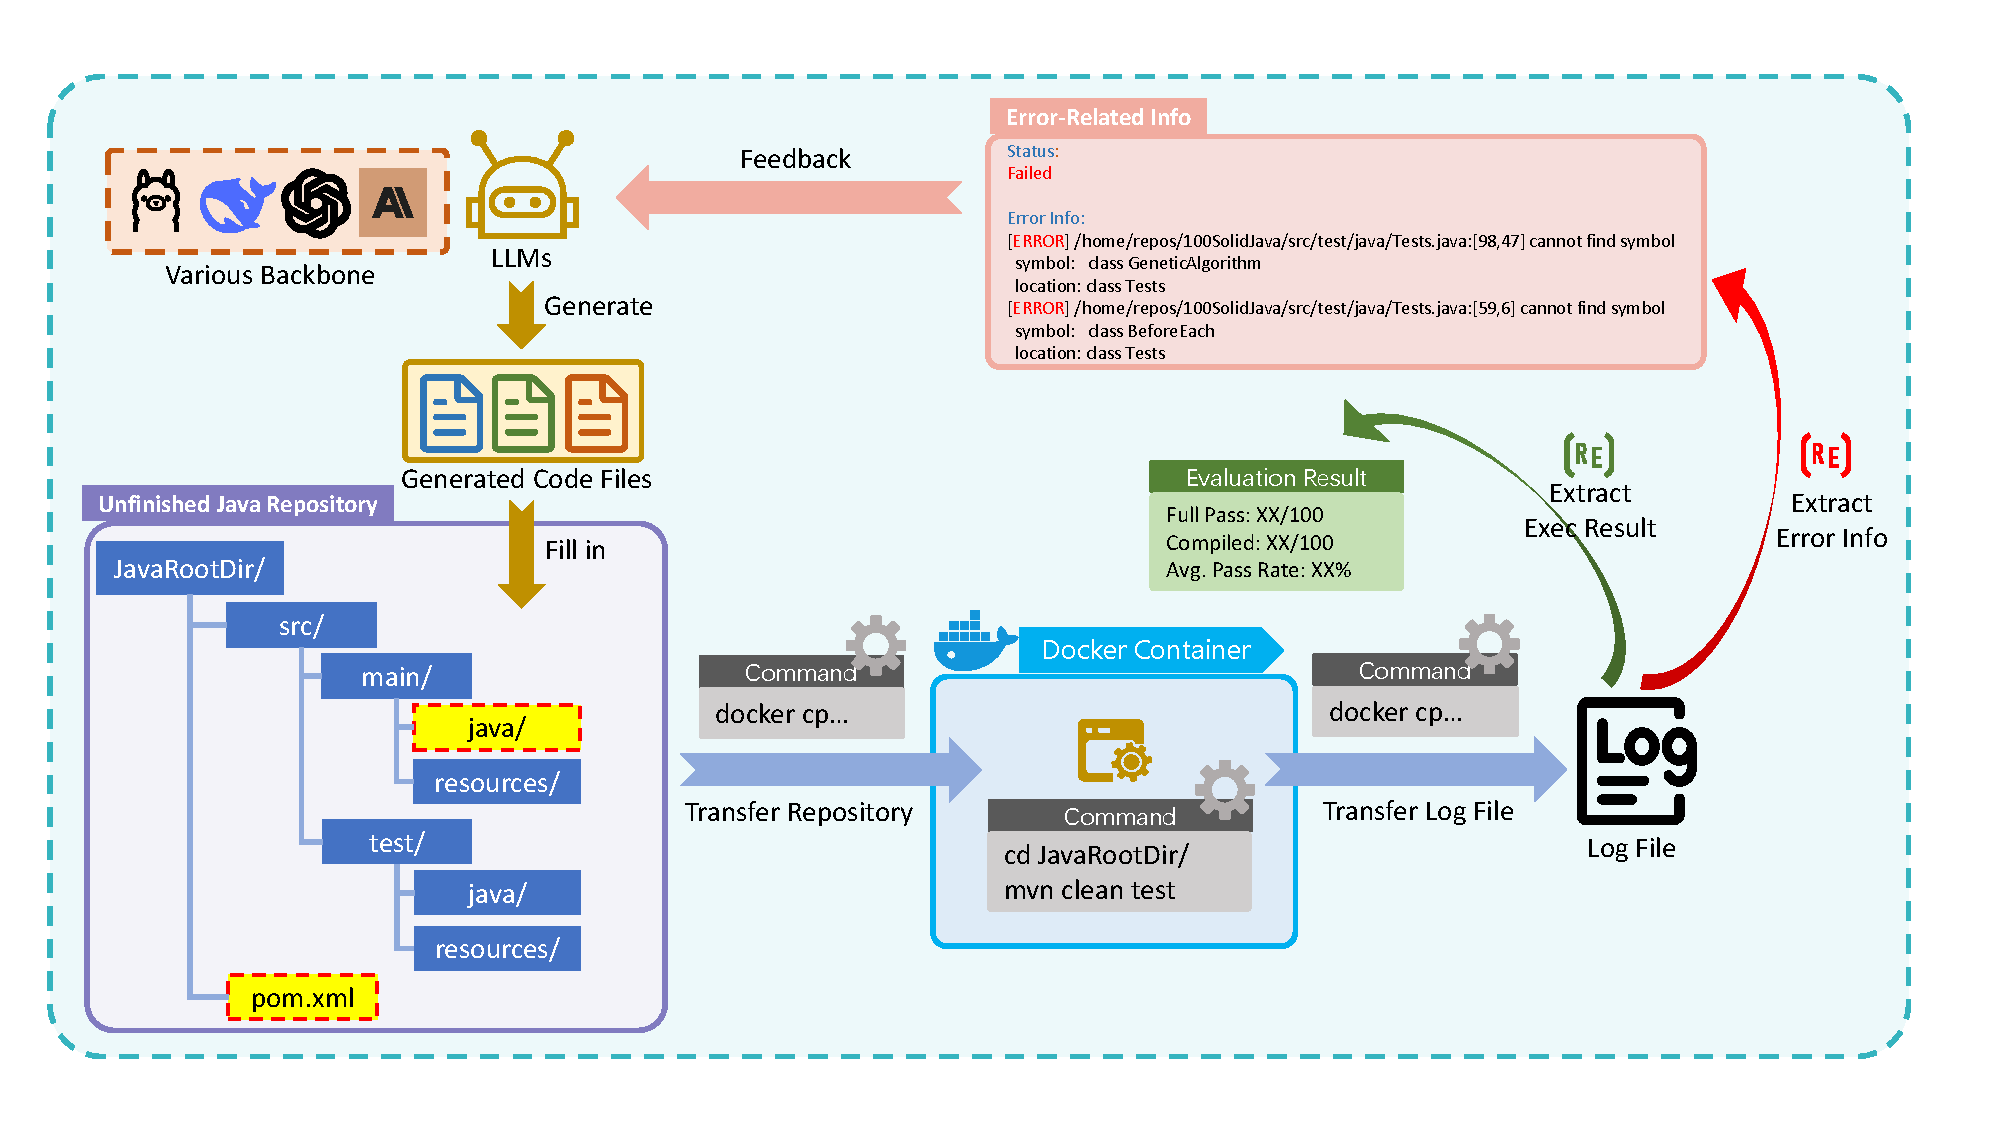
\includegraphics[width=\linewidth]{figures/EvaluationProcess.pdf}
%     % \vspace{-1em}
%     \caption{Overview of Evaluation Process.}
%    % \vspace{-0.5em}
%     \label{fig:EvaluationProcess}
% \end{figure}

\subsubsection{Evaluation Metrics}
Following previous studies~\cite{jimenez2023swe,tao2024magis,xia2024agentless}, we use these metrics to evaluate the performance of LLMs:
\begin{itemize}[left=10pt]
    \item \textbf{Resolve Rate:} the percentage of task instances that are resolved. 
    \item \textbf{Apply Rate:} the percentage of generated patches that are intergrated to codebase using Git~\cite{git} tool without any errors. 
    \item \textbf{Cost:} the average cost of evaluating task instances.
\end{itemize}
%\hy{is Rate a correct term here} \glh{we use the same term as SWE-bench.}



% \section{Evaluation}


%\hy{can the evaluation show that SWE-bench-X is better than SWE-bench in evaluating LLMs' ability in resolving github issure?} \glh{We attempt to prove two advantages. First, researchers can utilize our benchmark to evaluate the generalizability of their proposed methods in different languages. For example, the Agentless method, which is designed for Python language, show lower performance in JavaScript and TypeScript subset of our benchmark. We believe this is because this method does not consider some features of JS and TS, such as 'Interface'. Our benchmark can help them design methods applicable to multiple languages. Second, our benchmark contains important multi-modality data, which can be used to evaluate issue resolution ability of LLMs in a more real scenario. I am not sure if this is ok. }




% \subsubsection{Diverse issue type}

% We have observed that the collected instances are associated with a large number of issues, and these issues are often accompanied by certain labels. According to our understanding, many of the labels on GitHub are manually assigned. We collected data from 959 instances, which are associated with a total of 913 issues, out of which 735 issues have labels. In total, we gathered 1,742 labels.

% We invited two experienced software developers to categorize these labels, and they classified them into ten major categories, as shown in Table~\ref{table:labelsCategory}. Subsequently, the 1,742 labels were classified accordingly, and the results are displayed in Figure~\ref{fig:labelsDistribution}. It can be observed that the largest proportion of labels is related to the type of issue. These labels can help developers quickly understand the nature of the problem and are of significant value.

% \begin{table}[ht]
% \caption{Label Categories and Descriptions}
% \label{table:labelsCategory}
% \centering
% \footnotesize
% \begin{tabular}{ll}
% \toprule
% \textbf{Category Name} & \textbf{Description} \\
% \midrule
% \textbf{issue\_type} & Describes the type of issue like bug, feature, or documentation-related. \\
% % \hline
% \textbf{module\_component} & Identifies the module or component affected by the issue. \\
% % \hline
% \textbf{priority} & Specifies the urgency or importance of the issue or task. \\
% % \hline
% \textbf{language\_framework} & Denotes the programming language or framework related to the issue. \\
% % \hline
% \textbf{difficulty} & Indicates the difficulty level of a task, helpful for contributors. \\
% % \hline
% \textbf{status} & Represents the current status of the issue, such as waiting, closed, or active. \\
% % \hline
% \textbf{topic\_feature} & Relates the issue to a specific feature or topic in the project. \\
% % \hline
% \textbf{special\_misc} & Miscellaneous category for specialized or unclassified tags. \\
% % \hline
% \textbf{design\_api} & Labels related to system design, architecture, or API-specific tasks. \\
% % \hline
% \textbf{uncategorized} & Used for labels that don't fit other predefined categories. \\
% \bottomrule
% \end{tabular}

% \end{table}


% \begin{figure}[t]
%     \centering
%     % \vspace{-10pt}
%     
\includegraphics[width=0.6\linewidth]{ISSTA25-acmart-primary/figures/ClassfiedLabels.pdf}
%     % \vspace{-1em}
%     \caption{Distribution of different issue labels.}
%    % \vspace{-0.5em}
%     \label{fig:labelsDistribution}
% \end{figure}



% \begin{center}
%     \begin{myboxc} \textbf{RQ1 Summary: } \Swebenchx shows great diversity in programming languages, repository domains and modality of input information.
    
%     \end{myboxc} %cd
% \end{center}




% \subsection{Performance of LLMs }  
% In this section, we first evaluate issue resolution ability of three advanced LLMs on \Swebenchx with two methods.  And then we evaluate two LLMs with visual ability in SWE-bench-V.

\subsection{Performance of LLMs on \Swebenchx}
We evaluate three advanced LLMs with two methods on \Swebenchx. The results are presented in Table~\ref{table:performanceAll}. First, we can find that  performance of advanced LLMs on \Swebenchx remains limited. Among the evaluated models, \GPT with Agentless-X method achieves the highest resolve rate of 8.6\% and apply rate of 87.4\% on \Swebenchx. And \Claude with oracle retrieval method achieves the second best performance with the rate of 7.8\% and apply rate of 61.8\% on \Swebenchx. However, the performance of these LLMs across both methods remains limited,  highlighting the need for further improvements in the issue resolution ability of LLMs.


Second, the results show that the Agentless-X method outperforms the oracle retrieval method for both \GPT and \DeepSeek. Specifically, for \GPT-4, Agentless-X increases the resolve rate from 2.5\% to 8.6\% and the apply rate from 42.8\% to 87.4\%. Similarly, \DeepSeek's performance also improves with Agentless-X, as its resolve rate rises from 2.7\% to 3.9\%. These results demonstrate the effectiveness of Agentless method in improving the issue resolution ability of LLMs.

% For the Agentless-X method, we observe notable performance improvements for both \GPT and \DeepSeek compared to the oracle retrieval method. Specifically, \GPT’s resolve rate increases from 2.5\% to 8.6\%, and its apply rate rises from 42.8\% to 87.4\%. Similarly, \DeepSeek’s resolve rate improves from 2.7\% to 3.9\%. These results highlight the effectiveness of the Agentless method in enhancing performance across different languages.

Third, we find that \Claude performs better with the oracle retrieval method, achieving a resolve rate of 7.8\%, while its performance with the Agentless-X method is limited to only 1.9\%. We believe this higher performance with oracle retrieval is due to \Claude's strong capability in understanding long code segments, which allows it to make accurate code changes when the correct file locations are provided. In contrast, with Agentless-X method, \Claude's performance is limited because it often fails to produce results in the expected format during the localization stage. This inconsistency makes it hard to parse the location output correctly, ultimately preventing patch generation. The detailed discussion of this issue is in Section~\ref{sec:parseError}.


% We believe this is due to \Claude's strong capability in understanding long code, allowing it to generate accurate code changes when the correct file is identified through retrieval, resulting in better oracle retrieval performance. In contrast, with the Agentless method, we find that \Claude often fails to produce results in the expected format during the location phase, making it hard to parse the location output and ultimately preventing patch generation. The detailed discussion about this issue is shown in Section~\ref{sec:parseError}.  

% Last, we observe that the Agentless-X method performs 
% worse on JavaScript and TypeScript compared to Java and Python. We believe this is due to the method’s reliance on AST tools to extract and analyze file structures based on classes and methods. In languages like Python and Java, important information is typically organized within classes and methods, making AST-based extraction straightforward and effective. However, JavaScript and TypeScript present unique challenges. JavaScript often uses arrow functions and anonymous functions, which do not follow the traditional class and method structures and are thus difficult to identify and extract using AST alone. Additionally, in TypeScript, important information is often defined in types and interfaces, which are not covered by class and method extraction. To handle JavaScript and TypeScript more effectively, the Agentless-X method would need to account for these unique language features, such as arrow functions, anonymous functions, types, and interfaces.

Last, we observe that the Agentless-X method performs worse on JavaScript and TypeScript than on Java and Python. We believe this is due to the design of Agentless-X, which uses AST tools to parse repository files and locate key structures, such as classes and methods. In Python and Java, essential information is typically organized within classes and methods, so this AST-based extraction is effective. However, in JavaScript and TypeScript repositories, code frequently relies on types and interfaces to define important structures that are not part of the traditional class or method constructs. This makes it challenging for the original extraction method to capture this information effectively. Additionally, JavaScript and TypeScript always use anonymous and arrow functions, which AST tools struggle to parse compared to standard functions. For Agentless-X to handle JavaScript and TypeScript more effectively, it would need to account for these language-specific features, such as arrow functions, anonymous functions, and the use of types and interfaces.

% , categorized by programming language
\begin{table}[t]
  \centering
  \small %\footnotesize
  \setlength\tabcolsep{3pt}
  \caption{Performance comparison across different LLMs on \Swebenchx.}
  \tabmargin
  \label{table:performanceAll}
  \resizebox{\columnwidth}{!}{
    \begin{tabular}{ccccccc}
    \toprule
    \multirow{2}{*}{\textbf{Model}} & \multicolumn{3}{c}{\textbf{Oracle Retrieval}} & \multicolumn{3}{c}{\textbf{Agentless-X}} \\
    \cmidrule(r){2-4} \cmidrule(r){5-7}
    & \textbf{Resolve Rate} & \textbf{Apply Rate} & \textbf{Cost(\$)} & \textbf{Resolve Rate} & \textbf{Apply Rate} & \textbf{Cost(\$)} \\
    \midrule
    
    \textbf{DeepSeek-v2.5 (All)} & 2.7\% (26/959)  & 49.0\% (470/959) &  
    0.005& 3.9\% (37/959) & 52.0\% (499/959) & 0.010 \\
    \midrule
    \quad Python & 1.3\% (5/374) & 49.7\% (186/374)& 0.008 & 6.1\% (23/374)& 70.9\% (265/374)& 0.014 \\
    \quad TypeScript & 1.9\% (4/210)& 45.2\% (95/210)& 0.003 & 1.9\% (4/210)& 44.3\% (93/210)& 0.006 \\
    \quad JavaScript & 2.2\% (6/270)& 48.5\% (131/270)& 0.003 & 2.6\% (7/270)& 37.0\% (100/270) & 0.009 \\
    \quad Java & 10.5\%  (11/105)& 55.2\% (58/105) & 0.038 & 2.9\%  (3/105)&39.0\% (41/105)& 0.007 \\
    \midrule
    
    \textbf{\GPT (All)} & 2.7\% (26/959)  & 42.6\% (409/959) & 0.069 & \textbf{8.6\% (82/959)} & \textbf{87.4\% (838/959)} & 0.098 \\
    \midrule
    \quad Python &1.9\% (7/374) &42.5\% (159/374) & 0.112 & 8.8\% (33/374) & 89.3\% (334/374) & 0.090 \\
    \quad TypeScript & 3.3\% (7/210) &44.3\% (93/210) & 0.035 &6.2\% (13/210) &85.2\% (179/210) & 0.095 \\
    \quad JavaScript &1.9\% (5/270) & 40.0\% (108/270) & 0.049 &6.3\%  (17/270)&87.8\% (237/270) & 0.113 \\
    \quad Java &6.7\% (7/105)& 46.7\%  (49/105) & 0.003 & 18.1\% (19/105) &83.8\% (88/105) & 0.053 \\
    \midrule                                                 
    
    \textbf{\Claude (All)} &7.8\% (75/959) & 61.8\% (593/959) & 0.110 & 1.9\% 
 (18/959)& 14.6\%(140/959)& 0.272 \\
 % 17.6(169/959)& 0.272 \\
    \midrule
    \quad Python & 5.1\% (19/374) & 52.9\% (198/374) & 0.179 & 1.6\%  (6/374)& 1.6\% (55/374) &0.335 \\
 % (84/374)& 0.335 \\
    \quad TypeScript & 6.7\% (14/210) & 70.0\% (147/210) & 0.047 & 1.0\% (2/210) & 10.5\% 
 (22/210)& 0.170 \\
    \quad JavaScript & 8.5\%  (23/270)& 63.3\% (171/270) & 0.073 & 2.2\% (6/270)& 18.5\% (50/270) & 0.178 \\
    \quad Java & 18.1\% (19/105) & 73.3\% (77/105) & 0.063 &3.8\% (4/105|)& 12.4\% (13/105) & 0.342\\
    \bottomrule
    \end{tabular}
    }%

\end{table}

\begin{center} 
\begin{myboxc} \textbf{RQ1 Summary:} The performances of current LLMs remain limited on \Swebenchx. Besides, the Agentless-X method can effectively enhance issue resolution preformance of \GPT and \DeepSeek. However, while \Claude achieves good performance with the oracle retrieval method, it struggles with Agentless-X. Lastly, Agentless-X performs better on Java and Python compared to JavaScript and TypeScript. \end{myboxc} 
\end{center}

% \subsubsection{Performances in different languages.}\glh{maybe change this term to ``issues requiring image understanding''}
\subsection{Performances of LLMs on Issues With Visual Inputs }

We evaluate two advanced LLMs with visual understanding capabilities, \GPT and \Claude, on a set of 19 task instances that require understanding images in issues. This evaluation uses both oracle retrieval method and Agentless-X method. Additionally, given the relatively small size of the subset, we repeat each experiment three times to minimize the effects of randomness. To investigate the effect of visual inputs, we conduct experiments under three different settings: 

\begin{itemize}[left=10pt]
     \item \textbf{Text Only.} In this setting, we do not provide the actual images from issues to LLMs. Instead, we only include the image URLs as text, without any visual information.


    \item \textbf{Text \& Image.} In this setting, both the text and images from issues are input to LLMs. The LLMs use its visual capabilities to understand the images and resolve the issue.
    

 \item \textbf{Image-augmented Text.} This is a two-stage approach. In the first stage, we use a prompt to instruct models to understand images and to rewrite the issue text with visual information. In the second stage, the rewritten text, augmented with image details, is used as input to the model. Compared to the second setting, this approach allows us to better understand how the model processes and interprets the visual information. 
    



\end{itemize}

 The results are shown in Table~\ref{table:performanceVisual}, highlighting three key conclusions. First, current LLMs show limited performance on issues requiring image understanding. Using oracle retrieval method, which provides the correct files, \Claude achieves the best performance, resolving only 10.5\% of the issues in the image-augmented text setting. In contrast, \GPT performs poorly, resolving only 1.6\% of issues. Second, leveraging visual information is beneficial for resolving issues requiring image understanding. When using oracle retrieval method, compared to the ``Text only'' setting, \Claude's resolve rate increases from 3.5\% to 10.5\% in the ``Image-augmented Text'' setting. Third, LLMs with Agentless-X method struggle to resolve issues requiring image understanding.  Despite its solid performance on \Swebenchx, Agentless-X failed to resolve any issues requiring image understanding on both models. These results highlight  that current methods need improvements to utilize visual information effectively.

 



\begin{table}[t]
  \centering
  % \small
  \setlength{\tabcolsep}{2pt}
    \caption{Performance comparison across different LLMs on \Swebenchx-V.}
  \label{table:performanceVisual}
  \tabmargin
  \resizebox{\columnwidth}{!}{
    \begin{tabular}{llcccccc}
    \toprule
    \multirow{2}{*}{\textbf{Model}} & \multirow{2}{*}{\textbf{Setting}} & \multicolumn{3}{c}{\textbf{Oracle Retrieval}} & \multicolumn{3}{c}{\textbf{Agentless-X}} \\
    \cmidrule(r){3-5} \cmidrule(r){6-8}
    & & \textbf{Resolve Rate} & \textbf{Apply Rate} & \textbf{Cost(\$)} & \textbf{Resolve Rate} & \textbf{Apply Rate} & \textbf{Cost(\$)} \\
    \midrule
    \multirow{3}{*}{\GPT} 
    & Text Only & 1.6\% (1/57) & 45.6\% (26/57) & 0.036 & 0\% (0/57) & 42.1\% (24/57) & 0.096\\
    & Text \& Images & 1.6\% (1/57) & 33.3\% (19/57)  & 0.038 & 0\% (0/57) & 26.3\% (15/57) & 0.110\\
    & Images-agumented Text & 1.6\% (1/57) & 52.6\% (30/57) & 0.046 & 0\% (0/57) & 38.6\% (22/57) & 0.109\\
    \midrule
    \multirow{3}{*}{\Claude} 
    & Text Only & 3.5\% (2/57) & 50.9\% (29/57) & 0.058 & 0\% (0/57) & 57.9\% (33/57) &  0.210\\
    & Text \& Images & 3.5\% (2/57) & 59.6\% (34/57) & 0.062 & 0\% (0/57) & 63.2\% (36/57) &  0.224\\
    & Images-agumented Text & 10.5\% (6/57) &  59.6\% (34/57) & 0.074 & 0\% (0/57) & 52.6\% (30/57) & 0.233\\
    \bottomrule
    \end{tabular}
  }

\end{table}



\begin{center}
    \begin{myboxc} \textbf{RQ2 Summary: } %cd
     Our evaluation shows that current LLMs struggle with issues requiring image understanding. Besides,  leveraging visual information is beneficial for resolving issues requiring image understanding. However, we find LLMs with Agentless-X show limited performances on issues requiring image understanding, highlighting the need for methods to utilize visual information  effectively.
    \end{myboxc} %cd
\end{center}


 % First, resolving issues with images are more challenging, as seen in the lower resolve rates in SWE-bench-visual compared to Table~\ref{table:performanceAll}. Second, incorporating visual information is crucial for improving LLM performance on issues with images. For example, when images are added to the text input, \Claude's resolve rate increases from 3.51\% to 10.5\% in the oracle retrieval setting, indicating that visual context plays a vital role in resolving such issues. Finally, while the Agentless method performs well when handling text-only issues, it struggles significantly with issues that include images, indicating that further optimization is required to improve its effectiveness in visual contexts.


% \begin{table}[t]
%   \centering
%   \footnotesize
%   \setlength\tabcolsep{1.5pt}
%   \caption{Performance comparison across different LLMs on \Swebenchx.}
%   \label{table:performanceVisual}
%   % \vspace*{-10pt}
%   % \resizebox{\columnwidth}{!}{
%     \begin{tabular}{l|c|c|c|c|c|c|}
%     \hline
%     \textbf{Model} & \multicolumn{3}{c|}{\textbf{Oracle Retrieval}} & \multicolumn{3}{c|}{\textbf{Agentless-X}} \\
%     \cline{2-7}
   
%     & \textbf{Resolve Rate} & \textbf{Apply Rate} & \textbf{Cost(\$)} & \textbf{Resolve Rate} & \textbf{Apply Rate} & \textbf{Cost(\$)} \\
%    \hline
%     % Example Data
%     DeepSeek-v2.5 & 1.5\% & 48.3\% & 0.005 & 3.7\% & 46.3\% &  \\
%     \hline
%     \GPT & 1.7\%  & 42.6\% & 0.072 & 6.3\% & 63.0\% &  \\
%     \hline
%     claude-3.5-sonnet& 6.2\% & 60.0\% & 0.115 & 1.3\% & 10.9\% &  \\

%     \hline
%     \end{tabular}
%     % }%
 

\subsection{Failure Analysis}
To investigate why LLMs fails to resolve issues on \Swebenchx, we conduct an analysis and find two specific types of failures as follows.

% To further analyze why LLMs fail to resolve issues on \Swebenchx, we conduct an analysis and find two types of failure as follows.

\textbf{Parsing failure of structural output.} \label{sec:parseError}
This type of failure occurs in the localization stage of the Agentless-X method when the model fails to follow the specified output format given in the prompt. 
% In the Agentless-X method, the prompt requires the model to return the locations to be modified (e.g., class, function, and line numbers) and to wrap these results using code blocks as shown in Figure~\ref{fig:ErrorFormat}. These code blocks are critical for the correct parsing of the results, as a regular expression is applied to extract the relevant information.
 % This information must be enclosed in code blocks to ensure it can be extracted correctly.
In the example shown in Figure~\ref{fig:ErrorFormat}, the prompt instructs LLMs to provide the locations to be edited (e.g., class names, function names, method names, and line numbers) and to wrap these results with a code block. Then, this method uses regex expressions to parse the localization results from responses of LLMs. We can find that both \GPT and \DeepSeek follow the prompt's instructions, successfully enclosing their output in code blocks, allowing the results to be parsed correctly and used in the following repair stage. However, \Claude does not follow this format; instead of enclosing the location information in a code block, it provides the output in plain text, which leads to a parsing failure. As a result, no location information is passed to the repair stage, and no patch can be generated from \Claude in the following repair stage.  

To further explore the impact of this error, we compute the parsing success rate for each model in the localization stage of the Agentless-X framework, as shown in Table~\ref{table:ErrorFormatTable}. \GPT achieves the highest parsing success rate at 97.2\%, while \Claude obtains a much lower success rate of 11.8\%. This parsing error significantly affects \Claude's ability to generate patches, leading to a lower overall resolve rate (1.9\%). However, we find that this failure can be mitigated effectively by adding format constraints in original prompt. In our experiments, we append the original prompt with ``You must wrap the results with \verb|```|''. We find this prompt increases the \Claude's parsing success rate and hence increases the resolve rate from 1.9\% to 7.4\%. This results highlight the importance of building robust prompts in current methods.

 % `` You must wrap returned results with``` '' 
\begin{figure}[t]
    \centering
    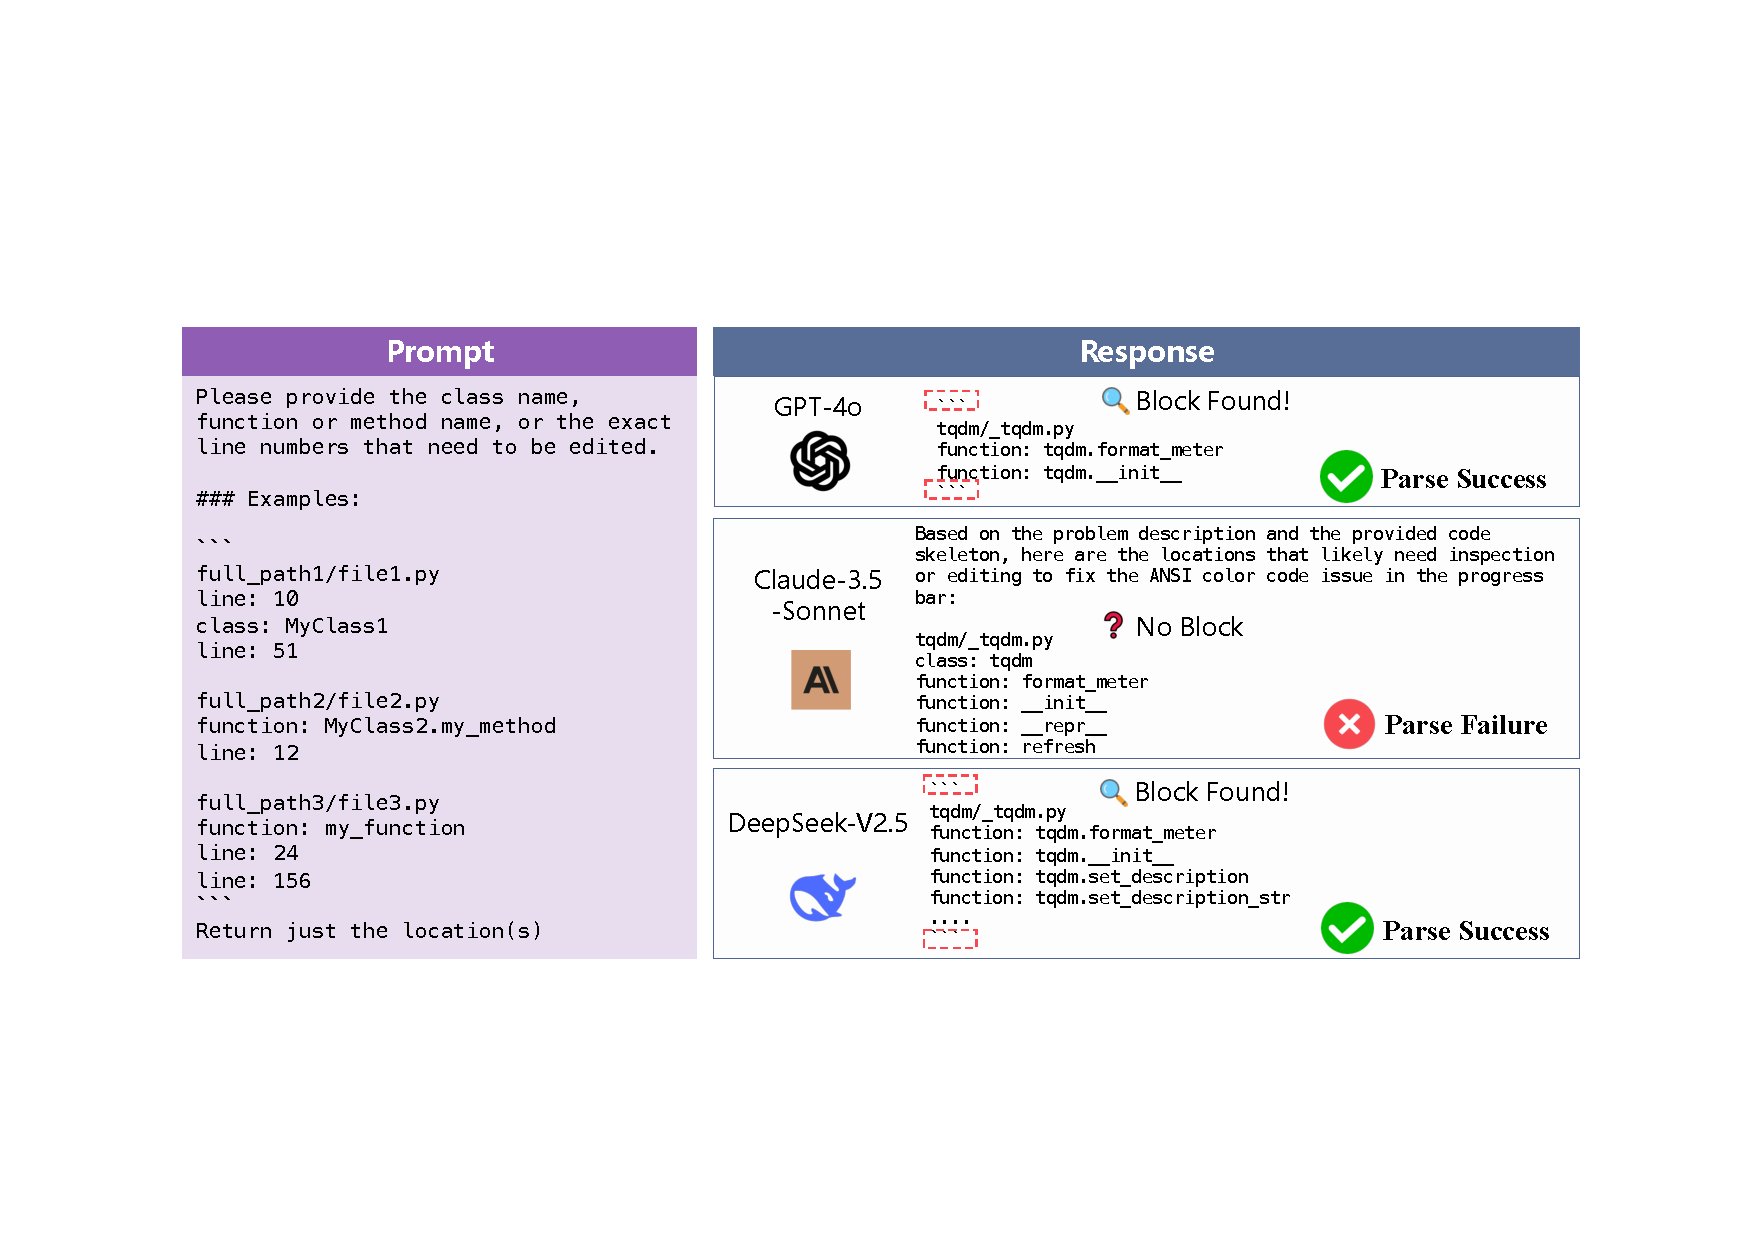
\includegraphics[width=0.9\linewidth]{figures/ErrorFormatV4.pdf}
    \figmargin
    \caption{Responses of different LLMs in the localization stage of Agentless-X. }
    \label{fig:ErrorFormat}
\end{figure}

\begin{table}[t]
  \centering
  \small % \footnotesize
  % \setlength\tabcolsep{1.5pt}
   \caption{Parsing success rate of LLMs with the Agentless-X method on \Swebenchx.}
  \label{table:ErrorFormatTable}
  \tabmargin
  % \vspace*{-10pt}
  % \resizebox{0.6\columnwidth}{!}{
    \begin{tabular}{lcccc}
    \toprule
    \multirow{2}{*}{\textbf{Model}} & \multicolumn{4}{c}{\textbf{Agentless-X}}  \\
    \cmidrule(r){2-5}
   
    &\textbf{Prompt Setting} & \textbf{Parsing success Rate} & \textbf{Resolve Rate} & \textbf{Apply Rate}  \\
   \midrule
    % Example Data

    \GPT & default &97.2\% (932/959) &8.6\% (82/959) & 87.4\% (838/959)  \\
    % \hline
    % \GPT(vision)  & 4.2\% &45.8\%  & 0.072 & 8.3\% & 83.3\% &  \\
    % \hline
    \DeepSeek & default& 82.5\% (791/959)  & 3.9\% (37/959) & 52.2\% (501/959)  \\
    % \hline
    \Claude & default & 10.0\% (96/959) &   1.9\% (18/959) &  17.6\% (169/959)   \\
    \Claude & new prompt & 98.5\% (945/959) &  7.4\% (71/959)  & 63.3\% (607/959) \\  
     
    \bottomrule
    \end{tabular}
    % }%

  % \vspace*{-2em}
\end{table}

\textbf{Insufficient ability of cross-file issue resolution.} In the issue resolution task, resolving issues that require modifications across multiple files is particularly challenging. To investigate LLMs' ability to resolve single-file and cross-file issues, we categorize issues on \Swebenchx into these two types.  For each issue, we use its gold patch as a reference and check how many files need to be modified to resolve the issue. If multiple files are modified in the gold patch of the issue, we classify this issue as a cross-file issue; otherwise, it is categorized as a single-file issue. And then we analyze performances of LLMs in two types of issues. As shown in Table~\ref{table:CrossFileEval}, we can observe that LLMs perform significantly worse on cross-file issues compared to single-file issues.  

We assume one reason LLMs perform poorly on cross-file issues is their tendency to modify only a single file. To investigate this assumption, we first examine the number of files modified in the patches generated by LLMs for cross-file issues. Then, we calculate the proportion of patches that include modifications to multiple files versus those with changes to only a single file. We find that, even with the oracle retrieval method, which provides the relevant files to the model, LLMs still primarily edit a single file. Specifically, \Claude modifies a single file in 88\% of issues, \GPT in 87\%, and \DeepSeek in 93\%. Moreover, with the Agentless-X method, all models modify a single file in 100\% of issues. These results highlight the insufficient ability of current LLMs in resolving issues that require modifying multiple files.

% The results are shown in Figure~\ref{fig:CrossFileEval}. Notably, even with the oracle retrieval method, which provides the relevant files to the model, LLMs still tend to edit a signle file. As shown in Figure~\ref{fig:
% }, \Claude modifies a single file in 78\% of issues, \GPT in 72\%, and \DeepSeek in 90\%. Moreover, under the Agentless-X method, all models only edit one file in 100\% of issues. 

% In the cross-file issue setting, we measure the proportion of cases where models only edited a single file. As shown in Figure~\ref{fig:CrossFileEval}, for the oracle retrieval method, the models tend to overwhelmingly edit just one file: \Claude edits a single file in 78\% of cases, \GPT in 72\%, and \DeepSeek in 90\% of cases.  However, when using the Agentless-X method, all models edited only one file in 100\% of cases. This result suggests that the LLMs sturggle to edit multiple files. It is crucial to enhance this capability for cross-file issues.

% on \Swebenchx based on the number of files edited in the gold patch. If the gold patch modifies multiple files, we consider the issue as a cross-file issue; otherwise, we consider the issue as a single-file issue. 

\begin{table}[t]
  \centering
  \small %\footnotesize
  \setlength\tabcolsep{4pt}
      \caption{Performance comparison across different LLMs on \Swebenchx for cross-file and single-file issues.}
  \label{table:CrossFileEval}
  \tabmargin
  % \resizebox{0.8\columnwidth}{!}{
    \begin{tabular}{llcccc}
    \toprule
    \multirow{2}{*}{\textbf{Model}} & \multirow{2}{*}{\textbf{Method}} & \multicolumn{2}{c}{\textbf{Single-file Issues}} & \multicolumn{2}{c}{\textbf{Cross-file Issues}} \\
    \cmidrule(r){3-4} \cmidrule(r){5-6}
    & & \textbf{Resolve Rate} & \textbf{Apply Rate} & \textbf{Resolve Rate} & \textbf{Apply Rate} \\
    \midrule
    \multirow{2}{*}{\GPT} 
    & Oracle Retrieval & 3.5\% (21/601) & 42.9\% (258/601) & 1.4\% (5/358) & 42.2\% (151/358) \\
    & Agentless-X &  12.0\% (72/601) & 87.4\% (525/601) & 2.8\% (10/358)  & 87.4\% (313/358) \\

    \midrule
    \multirow{2}{*}{\DeepSeek} 
    & Oracle Retrieval & 3.7\% (22/601)  & 50.6\% (304/601) & 1.1\% (4/358)  & 46.4\% (166/358) \\
    & Agentless-X & 5.2\% (31/601)  & 52.4\% (315/601) & 1.7\% (6/358)  & 51.4\% (184/358)  \\

    \midrule
    \multirow{2}{*}{\Claude} 
    & Agentless-X & 2.5\% (15/601) & 13.6\% (82/601) & 0.8\% (3/358) & 16.2\% (58/358) \\
    & Oracle Retrieval & 10.5\% (63/601) & 66.1\% (397/601) & 3.4\% (12/358) & 54.7\% (196/358) \\
    \bottomrule
    \end{tabular}
    % }%
    

\end{table}

% \begin{figure}[t]
%     \centering
%     % \vspace{-10pt}
%     
\includegraphics[width=0.75\linewidth]{ISSTA25-acmart-primary/figures/CrossFileEval.pdf}
%     % \vspace{-1em}
%     \caption{Responses of different LLMs in the location stage of Agentless-X. \hy{not necessary?}\hy{can try to use simple texts, no figures or table}\glh{to do}}
%    % \vspace{-0.5em}
%     \label{fig:CrossFileEval}
% \end{figure}

\begin{center}
    \begin{myboxc} \textbf{RQ3 Summary: } Our analysis shows that \Claude struggles to generate results in the expected format during the Agentless-X localization stage, leading to poor issue resolution performance. We find that adding specific format instructions to the prompt can improve \Claude's results. Additionally, current LLMs perform poorly on cross-file issues and tend to modify only a single file, even when multiple files require changes.
    \end{myboxc} %cd
\end{center}

\secmargin
\section{Threats to Validity}
A potential threat to validity is that the number of task instances in Java is relatively lower than in other languages. Note that \Swebenchx is an evolving benchmark, and in the future we plan to collect additional task instances covering more repositories, domains, and languages. Additionally, we only evaluate  LLMs with the oracle retrieval method and the Agentless method on \Swebenchx, as these methods are relatively straightforward to implement, especially given that most existing methods are not designed with multilingual support. In the future, we aim to evaluate more methods on \Swebenchx. Additionally, we do not evaluate the impact of website links on the issue resolution performance of LLMs in our dataset. This is because current issue resolution methods do not support interaction between LLMs and websites.
% A potential threat to the validity of the results is the inconsistency in LLMs' performance. To mitigate this, conducting 3 rounds of experiments can more accurately reflect the true performance of the LLMs. Regarding the issue of data leakage, our target test cases are translated from the source language, and the repository in the target language does not exist in the training data of the LLMs. Therefore, there is no risk of data leakage.
%\hy{write some more here} \glh{revised}

\secmargin
\section{Conclusion}

In this paper, we propose \Swebenchx, a GitHub issue resolution benchmark with multi-aspect
diversity in programming languages, repository domains and modality of input information. The evaluation results demonstrate that current LLMs show limited performances on \Swebenchx. Besides, we also find that current LLMs struggle to resolve issues that require understanding images. Furthermore, we analyze the reasons behind LLM's failure on \Swebenchx, to shed light on future performance improvements of LLMs on \Swebenchx. 

\secmargin
\section{Data Availability}
\label{sec:open-science}
Our tool and experimental data are available at our project \url{https://anonymous.4open.science/r/OmniGIRL}.


%\hy{need to add some more references}\glh{to do}
